% !TEX program = xelatex

\documentclass{uetgraduation}
\usepackage{enumitem}
\usepackage{listings}
\usepackage{color}
\usepackage{url}
\usepackage{hyperref}
\usepackage{booktabs}
\usepackage{tabularx}
\usepackage{array}
\usepackage{float}
\usepackage{multirow}
\definecolor{codegreen}{rgb}{0,0.6,0}
\definecolor{codegray}{rgb}{0.5,0.5,0.5}
\definecolor{codepurple}{rgb}{0.58,0,0.82}
\definecolor{backcolour}{rgb}{0.95,0.95,0.92}


\begin{document}
\setlist[itemize]{left=2cm}
\lstset{
    language=Python,
    backgroundcolor=\color{backcolour},   
    commentstyle=\color{codegreen},
    keywordstyle=\color{magenta},
    numberstyle=\tiny\color{codegray},
    stringstyle=\color{codepurple},
    basicstyle=\ttfamily\footnotesize,
    breakatwhitespace=false,         
    breaklines=true,                 
    captionpos=b,                    
    keepspaces=true,                 
    numbers=left,                    
    numbersep=5pt,                  
    showspaces=false,                
    showstringspaces=false,
    showtabs=false,                  
    tabsize=2
}

\studentname{Trần Duy Hưng}
\title{PHÁT TRIỂN AI AGENTS \\ PHÁT HIỆN BỆNH TRÊN LÁ LÚA}
\documenttype{Đồ án tốt nghiệp đại học chính quy}
\major{Kỹ thuật máy tính}
\year{2026}
\supervisor{TS. Phạm Duy Hưng}

\makecovers

\begin{preamble}{Tóm tắt}
\addcontentsline{toc}{chapter}{Tóm tắt}
\textbf{Tóm tắt:} Đồ án này trình bày quá trình xây dựng một hệ thống chẩn đoán bệnh cây lúa ứng dụng kiến trúc Đa Tác Nhân (Multi-Agent System). Xuất phát từ thực tế nông dân vùng sâu vùng xa khó tiếp cận chuyên gia nông nghiệp, đề tài hướng đến việc cung cấp công cụ chẩn đoán tự động, có thể sử dụng qua thiết bị di động có kết nối Internet. Bốn loại bệnh được hỗ trợ là Đạo ôn (\textit{Rice Blast}), Bạc lá (\textit{Bacterial Blight}), Đốm nâu (\textit{Brown Spot}) và Vàng lùn (\textit{Tungro}).

Về mặt kỹ thuật, hệ thống gồm năm Agent chuyên biệt: Preprocessing Agent (tiền xử lý ảnh), Classification Agent (phân loại bệnh bằng Vision Transformer), Morphology Agent (phân tích hình thái bằng Gemini Vision), Retrieval Agent (tra cứu tri thức từ ChromaDB), và Coordinator Agent (tổng hợp báo cáo). Mô hình ViT được sử dụng trực tiếp qua Hugging Face mà không cần huấn luyện lại, nhờ đó tiết kiệm tài nguyên tính toán đáng kể. Cơ chế RAG với ChromaDB được đưa vào để đảm bảo các khuyến nghị điều trị được tham chiếu từ tri thức có kiểm chứng, hạn chế hiện tượng ``ảo giác'' của mô hình ngôn ngữ lớn.

Giao diện người dùng được xây dựng bằng Streamlit, API backend sử dụng FastAPI, và toàn bộ hệ thống được đóng gói bằng Docker. Trong quá trình thực hiện, một số khó khăn đã gặp phải như latency cao của Gemini API ($\approx 8$--$10$ giây mỗi lần gọi) và yêu cầu bộ nhớ lớn khi tải mô hình ViT lên CPU. Kết quả đánh giá cho thấy hệ thống đạt F1-score trung bình $\geq 0.96$ trên tập kiểm thử, thời gian phản hồi trung bình khoảng $14$--$15$ giây cho một lần chẩn đoán hoàn chỉnh.

\vspace{0.5cm}
\noindent \textit{\textbf{Từ khóa:} Vision Transformer, Multi-Agent System, RAG, ChromaDB, Gemini, FastAPI, Streamlit, Bệnh cây lúa.}
\end{preamble}
\clearpage
\addcontentsline{toc}{chapter}{Lời cam đoan}

\begin{center}
    \textbf{\fontsize{13pt}{19pt}\selectfont LỜI CAM ĐOAN}
\end{center}
\vspace{0.5cm}

Em xin cam đoan đây là công trình nghiên cứu của riêng em dưới sự hướng dẫn của giảng viên. Các nội dung nghiên cứu, kết quả phân tích trong đồ án là hoàn toàn trung thực, khách quan và chưa từng được công bố trong bất kỳ công trình nào khác. Em không sao chép các tài liệu, dự án hoặc công trình nghiên cứu của tác giả khác mà không chỉ rõ trong phần tài liệu tham khảo. Tất cả các mô hình, số liệu và thuật toán lập trình đều được xây dựng dựa trên sự hiểu biết và áp dụng công nghệ khoa học thực tế. Nếu phát hiện có sự sao chép vi phạm bản quyền hay vi phạm đạo đức học thuật, em xin hoàn toàn chịu trách nhiệm trước Hội đồng nhà trường.

\vspace{1.5cm}
\hfill
\begin{minipage}{0.4\textwidth}
\centering
\textit{Hà Nội , ngày ...... tháng ...... năm 2026} \\[1cm]
\textbf{Sinh viên thực hiện}\\(Ký và ghi rõ họ tên) \\[2cm] \textbf{Trần Duy Hưng}
\end{minipage}
\clearpage

% ─────────────────────────────────────────────
% 3. LỜI CẢM ƠN
% ─────────────────────────────────────────────
\addcontentsline{toc}{chapter}{Lời cảm ơn}

\begin{center}
    \textbf{\fontsize{13pt}{19pt}\selectfont LỜI CẢM ƠN}
\end{center}
\vspace{0.5cm}

Lời đầu tiên, em xin gửi lời cảm ơn đến Khoa Điện tử Viễn thông, Trường Đại học Công nghệ, Đại học Quốc Gia Hà Nội đã hỗ trợ, tạo điều kiện tốt nhất cho em để hoàn thành khóa luận tốt nghiệp này.

Em cũng xin được bày tỏ lòng biết ơn sâu sắc tới thầy TS. Phạm Duy Hưng đã dành thời gian quý báu, tận tình hướng dẫn, đóng góp những ý kiến xác đáng để em có thể hoàn thành khóa luận một cách tốt nhất.

Cuối cùng, em xin gửi lời cảm ơn sâu sắc đến các thầy cô giảng viên Trường Đại học Công nghệ, Đại học Quốc Gia Hà Nội đã luôn luôn chỉ dạy và giúp đỡ em, đặt cho em nền tảng vững chắc để có thể phát triển trong ngành Kỹ thuật Máy tính. Em cũng xin cảm ơn gia đình và bạn bè đã chăm sóc, giúp đỡ, làm chỗ dựa tinh thần to lớn cho em vượt qua những khó khăn trong quá trình học tập.

Do thời gian có hạn, kinh nghiệm còn hạn chế, khóa luận tốt nghiệp không tránh khỏi những thiếu sót. Em rất mong nhận được sự đóng góp của các thầy cô giảng viên để khóa luận được hoàn thiện hơn.

Em xin chân thành cảm ơn!

\clearpage

\begin{contentlisting}

\tableofcontents

\listoffigures
\listoftables

\begin{contentlistingsection}{Các từ viết tắt}
AI - Artificial Intelligence: Trí tuệ nhân tạo

Agent - AI Agent: Tác nhân trí tuệ nhân tạo

API - Application Programming Interface: Giao diện lập trình ứng dụng

ASGI - Asynchronous Server Gateway Interface

CNN - Convolutional Neural Network: Mạng nơ-ron tích chập

CLS - Classification Token: Token phân loại đặc biệt trong ViT

CORS - Cross-Origin Resource Sharing

CPU - Central Processing Unit: Bộ xử lý trung tâm

DB - Database: Cơ sở dữ liệu

DL - Deep Learning: Học sâu

FFN - Feed-Forward Network: Mạng truyền thẳng

GELU - Gaussian Error Linear Unit: Hàm kích hoạt GELU

GPU - Graphics Processing Unit: Bộ xử lý đồ họa

HTTP - Hypertext Transfer Protocol

LLM - Large Language Model: Mô hình ngôn ngữ lớn

MAS - Multi-Agent System: Hệ thống đa tác nhân

ML - Machine Learning: Học máy

MLP - Multi-Layer Perceptron: Perceptron đa lớp

MHSA - Multi-Head Self-Attention: Chú ý bản thân đa đầu

NLP - Natural Language Processing: Xử lý ngôn ngữ tự nhiên

PNG - Portable Network Graphics: Định dạng ảnh PNG

RAG - Retrieval-Augmented Generation: Tìm kiếm tăng cường bằng truy xuất

REST - Representational State Transfer

RGB - Red-Green-Blue: Không gian màu RGB

UI - User Interface: Giao diện người dùng

ViT - Vision Transformer: Bộ biến đổi thị giác

\end{contentlistingsection}

\begin{contentlistingsection}{Các ký hiệu toán học}

$Q, K, V$ - Query, Key, Value matrices: Ma trận Query, Key, Value trong cơ chế Attention

$d_k$ - Key Dimension: Chiều không gian của vector khóa

$\mathbf{A}, \mathbf{B}$ - Embedding Vectors: Các vector nhúng

$\cos(\theta)$ - Cosine Similarity: Độ tương đồng cosine giữa hai vector

$\hat{y}$ - Predicted Label: Nhãn dự đoán của mô hình

$\sigma(\cdot)$ - Sigmoid Function: Hàm sigmoid

$\text{softmax}(\cdot)$ - Softmax Function: Hàm softmax chuẩn hóa xác suất

$\mathcal{L}$ - Loss Function: Hàm mất mát

$\nabla$ - Gradient Operator: Toán tử gradient

$\|\cdot\|$ - Euclidean Norm (L2 Norm): Chuẩn Euclidean

\end{contentlistingsection}
\end{contentlisting}
\begin{center}
    \textbf{\fontsize{16pt}{19pt}\selectfont Mở đầu}
\end{center}
\vspace{0.5cm}
\addcontentsline{toc}{chapter}{Mở đầu}

\textbf{Tính cấp thiết của đề tài:} Việt Nam là quốc gia xuất khẩu gạo lớn thứ ba thế giới, với sản lượng đạt 43.5 triệu tấn thóc năm 2022 và kim ngạch xuất khẩu hơn 3.5 tỷ USD. Lúa gạo không chỉ là mặt hàng xuất khẩu chủ lực mà còn là nguồn thu nhập trực tiếp của hàng triệu hộ nông dân, đặc biệt ở Đồng bằng sông Cửu Long và Đồng bằng sông Hồng \cite{fao2023}. Tuy nhiên, năng suất lúa thường xuyên bị đe dọa bởi bệnh hại. Theo FAO, riêng bệnh Đạo ôn hàng năm gây thiệt hại tương đương lượng gạo đủ nuôi sống 60 triệu người \cite{valent1991}. Bốn loại bệnh phổ biến nhất --- Đạo ôn, Bạc lá, Đốm nâu và Tungro --- có thể làm giảm năng suất từ 20\% đến 100\% nếu không được phát hiện sớm. Điểm mấu chốt là: bệnh lúa chỉ có thể điều trị hiệu quả trong vài ngày đầu bùng phát; để quá 5--7 ngày, nông dân có thể mất toàn bộ vụ mùa. Vấn đề là việc chẩn đoán đúng loại bệnh đòi hỏi kinh nghiệm thực địa nhiều năm, trong khi số lượng cán bộ khuyến nông ngày càng không đủ đáp ứng nhu cầu tại vùng sâu vùng xa. Nông dân thường phải chờ nhiều ngày để được tư vấn, hoặc phải phun thuốc theo kinh nghiệm --- dẫn đến lãng phí và ô nhiễm môi trường. Đây là vấn đề thực tế mà đề tài này hướng đến giải quyết.

\textbf{Ý nghĩa khoa học và thực tiễn:} Về mặt khoa học, đề tài thử nghiệm việc kết hợp ba hướng tiếp cận còn tương đối mới trong lĩnh vực nông nghiệp thông minh: thay thế CNN bằng Vision Transformer để tận dụng cơ chế attention toàn cục; sử dụng RAG để hạn chế hallucination khi LLM đưa ra khuyến nghị điều trị; và tổ chức các mô-đun AI thành kiến trúc đa tác nhân để dễ bảo trì và mở rộng. Sự kết hợp này, theo tìm hiểu của tác giả, chưa được áp dụng đồng bộ trong các nghiên cứu về bệnh học cây lúa tại Việt Nam. Về mặt thực tiễn, sản phẩm đầu ra là ứng dụng web đầy đủ chức năng: giao diện song ngữ Việt--Anh qua Streamlit, API backend qua FastAPI, và hạ tầng đóng gói Docker. Nông dân chỉ cần chụp ảnh lá lúa bằng điện thoại và tải lên để nhận báo cáo chẩn đoán bằng tiếng Việt trong vòng khoảng 15 giây.

\textbf{Đối tượng và phạm vi nghiên cứu:}
\\ \indent Đối tượng nghiên cứu:
\begin{itemize}[leftmargin=1.5cm]
    \item Hình thái các vết bệnh trên phạm vi cấu trúc lá lúa.
    \item Bộ dữ liệu ảnh lá lúa mắc bệnh từ Hugging Face.
    \item Kiến trúc mô hình Vision Transformer và kỹ thuật fine-tuning.
    \item Cơ chế Retrieval-Augmented Generation và cơ sở dữ liệu vector.
    \item Thiết kế hệ thống đa tác nhân cho bài toán phân tích ảnh nông nghiệp.
\end{itemize}

Phạm vi nghiên cứu:
\begin{itemize}[leftmargin=1.5cm]
    \item Bốn loại bệnh lúa: Đạo ôn, Bạc lá, Đốm nâu, Tungro.
    \item Ảnh đầu vào dạng JPG/PNG, kích thước tối thiểu $224 \times 224$ pixel.
    \item Triển khai trên môi trường Linux/MacOS với Python 3.12.
    \item Giao diện tiếng Việt, hướng đến người dùng tại Việt Nam.
\end{itemize}

\textbf{Phương pháp nghiên cứu:}
\begin{enumerate}[leftmargin=1.5cm]
    \item Nghiên cứu lý thuyết: Tổng hợp tài liệu về ViT, Multi-Agent System, RAG, LLM từ các bài báo khoa học và tài liệu kỹ thuật.
    \item Thiết kế kiến trúc hệ thống: Xây dựng sơ đồ kiến trúc microservice và mô hình Agent-based.
    \item Lập trình và tích hợp: Triển khai từng Agent, tích hợp các mô hình AI, xây dựng API và giao diện.
    \item Kiểm thử và đánh giá: Kiểm thử đơn vị (unit test) và tích hợp (integration test) bằng pytest; đánh giá độ chính xác trên tập dữ liệu chưa từng thấy (unseen validation set).
\end{enumerate}

\textbf{Cấu trúc đồ án:}
Đồ án được tổ chức thành ba chương chính:

\begin{itemize}[leftmargin=1.5cm]
    \item \textbf{Chương 1 --- Cơ sở lý thuyết:} Trình bày nền tảng lý thuyết về bệnh học cây lúa, mô hình CNN, Vision Transformer, mô hình ngôn ngữ lớn, kỹ thuật RAG và ChromaDB, cùng lý thuyết về hệ thống đa tác nhân.
    \item \textbf{Chương 2 --- Thiết kế và Kiến trúc hệ thống:} Mô tả chi tiết kiến trúc tổng thể, thiết kế từng Agent, thiết kế API RESTful và cơ sở dữ liệu vector.
    \item \textbf{Chương 3 --- Triển khai, Giao diện và Kiểm thử:} Đề cập đến môi trường triển khai Docker, giao diện người dùng Streamlit, phương pháp kiểm thử và phân tích kết quả thực nghiệm.
\end{itemize}
\clearpage
\chapter{Cơ sở lý thuyết}
\section{Tổng quan về bệnh hại trên cây lúa}
\subsection{Bối cảnh và tầm quan trọng}
Cây lúa (\textit{Oryza sativa}) là cây lương thực chủ yếu của hơn 3.5 tỷ người trên thế giới, đặc biệt ở các nước châu Á. Trong vòng đời sinh trưởng, cây lúa dễ bị tấn công bởi nhiều loại mầm bệnh từ nấm, vi khuẩn và virus, gây thiệt hại kinh tế ước tính hàng chục tỷ USD mỗi năm. Tại Việt Nam, diện tích canh tác lúa đạt 7.1 triệu héc-ta với ba vụ thu hoạch mỗi năm; điều kiện khí hậu nhiệt đới ẩm tạo môi trường lý tưởng cho nhiều loại nấm và vi khuẩn phát triển, đặc biệt trong giai đoạn đẻ nhánh và làm đòng.

\subsection{Bệnh Đạo ôn (Rice Blast)}
\textbf{Tác nhân:} Nấm \textit{Pyricularia oryzae} (hay còn gọi là \textit{Magnaporthe oryzae}). Chu kỳ lây nhiễm bắt đầu từ bào tử nấm bám vào bề mặt lá và xâm nhập qua khí khổng hoặc trực tiếp qua lớp biểu bì.

\textbf{Triệu chứng đặc trưng:}
\begin{itemize}[leftmargin=1.5cm]
    \item Vết bệnh có hình thoi hoặc hình mắt chim, kích thước 1--2 cm.
    \item Tâm vết bệnh màu xám nhạt, viền màu nâu đậm hoặc vàng.
    \item Giai đoạn nặng: vết bệnh lan ra toàn bộ lá, lá héo khô.
    \item Bệnh tấn công cả cổ bông (cổ gié), gây lép hạt nghiêm trọng.
\end{itemize}

\textbf{Điều kiện phát triển:} Độ ẩm không khí cao ($>90\%$), nhiệt độ $20$--$28^\circ$C, trời âm u có sương mù là môi trường thuận lợi nhất. Bón thừa đạm là nguyên nhân chính kích thích bệnh bùng phát.

\subsection{Bệnh Bạc lá (Bacterial Leaf Blight)}
\textbf{Tác nhân:} Vi khuẩn \textit{Xanthomonas oryzae pv. oryzae} --- một trong những tác nhân gây bệnh cây trồng nguy hiểm nhất thế giới. Vi khuẩn xâm nhập qua vết thương cơ học hoặc khí khổng, nhân lên nhanh chóng trong mô lá và tiết ra enzyme phá vỡ thành tế bào.

\textbf{Triệu chứng đặc trưng:}
\begin{itemize}[leftmargin=1.5cm]
    \item Dải vàng hoặc trắng bạc chạy dọc theo mép lá, từ chóp lá lan xuống.
    \item Ranh giới giữa vùng bệnh và vùng khỏe không rõ ràng, có dạng lượn sóng.
    \item Buổi sáng sớm có thể quan sát thấy giọt dịch vi khuẩn màu đục vàng nhạt đọng ở mép lá --- đây là dấu hiệu đặc trưng nhất để phân biệt bạc lá với các bệnh khác.
    \item Lá bệnh khô và cuộn lại từ mép vào trong.
\end{itemize}

\textbf{Điều kiện phát triển:} Nhiệt độ $28$--$32^\circ$C, độ ẩm cao, mưa to gió lớn là điều kiện lây lan mạnh nhất. Bệnh đặc biệt nghiêm trọng trong vụ hè thu tại Đồng bằng sông Cửu Long.

\subsection{Bệnh Đốm nâu (Brown Spot)}
\textbf{Tác nhân:} Nấm \textit{Bipolaris oryzae} (đồng danh \textit{Helminthosporium oryzae}). Đây là bệnh có lịch sử lâu đời nhất và liên quan đến nạn đói Bengal năm 1943, nơi bệnh đốm nâu phá hủy phần lớn mùa màng lúa ở Ấn Độ.

\textbf{Triệu chứng đặc trưng:}
\begin{itemize}[leftmargin=1.5cm]
    \item Vết bệnh hình tròn hoặc bầu dục, màu nâu đậm, kích thước bằng hạt vừng đến hạt đậu.
    \item Tâm vết bệnh có thể chuyển màu xám nhạt ở giai đoạn muộn, bao quanh bởi quầng vàng nhạt.
    \item Phân bố tản mạn, không theo hướng gân lá như bệnh bạc lá.
\end{itemize}

\textbf{Điều kiện phát triển:} Ruộng nghèo dinh dưỡng (thiếu Kali, Silic), đất phèn, ngộ độc hữu cơ. Nhiệt độ $16$--$36^\circ$C, độ ẩm $86$--$100\%$.

\subsection{Bệnh Vàng lùn --- Tungro}
\textbf{Tác nhân:} Phức hợp hai loại virus: \textit{Rice tungro spherical virus} (RTSV) và \textit{Rice tungro bacilliform virus} (RTBV). Đặc biệt, bệnh không lây trực tiếp từ cây sang cây mà phụ thuộc hoàn toàn vào vật trung gian là rầy xanh đuôi đen (\textit{Nephotettix virescens}).

\textbf{Triệu chứng đặc trưng:}
\begin{itemize}[leftmargin=1.5cm]
    \item Cây lúa bị lùn lại rõ rệt so với cây khỏe mạnh cùng lứa tuổi.
    \item Lá có màu vàng cam hoặc vàng nhạt, bắt đầu từ chóp lá lan dần xuống gốc.
    \item Khác với triệu chứng thiếu đạm, màu vàng do Tungro thường không đồng đều, lốm đốm.
    \item Số bông giảm, hạt lép nhiều, năng suất có thể giảm đến 100\%.
\end{itemize}

\textbf{Điều kiện phát triển:} Mật độ rầy xanh đuôi đen cao, đặc biệt trong điều kiện thời tiết nóng ẩm, nhiệt độ $25$--$30^\circ$C và độ ẩm không khí trên $80\%$. Ruộng gieo sạ dày, bón thừa đạm, canh tác liên tục nhiều vụ và còn lúa chét là điều kiện thuận lợi cho rầy phát sinh, lan truyền virus nhanh chóng.

\begin{table}[H]{So sánh đặc điểm nhận dạng bốn loại bệnh lúa phổ biến}
\centering
\small
\setlength{\tabcolsep}{4pt}
\begin{tabular}{>{\bfseries}p{2.6cm} p{3.2cm} p{3.2cm} p{3.2cm} p{3.2cm}}
\toprule
\textbf{Đặc điểm} & \textbf{Đạo ôn} & \textbf{Bạc lá} & \textbf{Đốm nâu} & \textbf{Vàng lùn} \\
\midrule
Tác nhân & Nấm \textit{P. oryzae} & Vi khuẩn \textit{X. oryzae} & Nấm \textit{B. oryzae} & \textit{RTSV, RTBV}\\[4pt]
Đặc điểm nhận dạng & Vết bệnh màu xám, viền nâu vàng, có hình thoi, mắt chim & Dải bệnh màu vàng, trắng & Vết bệnh màu nâu, có hình tròn, bầu dục & Cây lùn, vàng lá\\[4pt]
Phân bố & Rải rác trên lá & Dọc theo mép lá & Tản mạn toàn lá \\[4pt]
Điều kiện & Ẩm, mát, có sương & Nóng, ẩm, gió lớn & Đất nghèo dinh dưỡng & Mật độ rầy xanh cao, thời tiết nóng ẩm\\[4pt]
Nguy hiểm & Rất cao & Cao & Trung bình--cao & Cao\\
\bottomrule
\end{tabular}
\end{table}

\section{Tổng quan tình hình nghiên cứu}

\subsection{Các nghiên cứu sử dụng CNN trong phát hiện bệnh cây trồng}

Từ khoảng năm 2016, các mạng tích chập sâu (CNN) bắt đầu được áp dụng rộng rãi vào bài toán nhận dạng bệnh cây trồng qua ảnh. Mohanty et al. (2016) \cite{mohanty2016} là một trong những nghiên cứu tiên phong, sử dụng mạng AlexNet và GoogLeNet để phân loại 26 loại bệnh trên 14 loại cây, đạt độ chính xác 99.35\% trên tập kiểm thử từ bộ dữ liệu PlantVillage. Tuy nhiên, bộ dữ liệu này được chụp trong điều kiện phòng thí nghiệm --- nền đồng nhất, ánh sáng kiểm soát --- nên khi áp dụng vào điều kiện thực địa, hiệu năng sụt giảm đáng kể do nền phức tạp, ánh sáng thay đổi và góc chụp không nhất quán.

Riêng với cây lúa, Sethy et al. (2020) \cite{sethy2020} đề xuất phương pháp kết hợp CNN để trích xuất đặc trưng và SVM để phân loại, đạt 98.33\% trên tập dữ liệu lá lúa. Jiang et al. (2019) \cite{jiang2019} thử nghiệm ResNet-50 trên ảnh bệnh lúa thu thập tại Trung Quốc và nhận xét rằng khả năng mô hình hóa các phụ thuộc tầm xa là hạn chế lớn nhất của CNN khi xử lý các vết bệnh phân bố không đồng đều trên lá. Đây cũng là động lực chính để tác giả chuyển sang kiến trúc Vision Transformer trong đề tài này.

Điểm chung của các nghiên cứu CNN là: hiệu năng cao trên tập kiểm thử nhưng dễ suy giảm khi gặp ảnh thực địa, khó giải thích quyết định phân loại, và thường chỉ dừng ở bước phân loại mà không tích hợp thêm tri thức bệnh học hay khuyến nghị điều trị.
\newpage
\subsection{Ứng dụng Vision Transformer trong nhận dạng bệnh cây trồng}

Sau khi Dosovitskiy et al. (2021) \cite{dosovitskiy2020} chứng minh ViT có thể cạnh tranh với CNN trên ImageNet khi có đủ dữ liệu tiền huấn luyện, nhiều nhóm nghiên cứu đã thử nghiệm ViT cho bài toán bệnh cây trồng. Chen et al. (2021) \cite{chen2021} so sánh ViT-Base với ResNet-50 trên tập dữ liệu PlantVillage và cho thấy ViT vượt trội 2--3\% F1-score, đặc biệt trên các lớp bệnh có hình thái phức tạp như đốm vòng và thối nhũn.

Saleem et al. (2022) \cite{saleem2022} ứng dụng ViT kết hợp với Grad-CAM để trực quan hóa vùng lá mà mô hình chú ý nhiều nhất, giúp tăng tính giải thích. Nghiên cứu này chỉ ra rằng ViT có xu hướng tập trung vào biên của vết bệnh --- nơi ranh giới giữa mô khỏe và mô bệnh rõ ràng nhất --- trong khi CNN thường kích hoạt trên vùng trung tâm vết bệnh.

Đối với lúa cụ thể, Islam et al. (2022) \cite{islam2022} fine-tune ViT-Base trên bộ dữ liệu gồm 5 loại bệnh lúa thu thập tại Bangladesh, đạt F1 = 0.961 --- gần với kết quả của đề tài này (F1 = 0.963). Điểm khác biệt là nghiên cứu đó dừng lại ở bước phân loại; đề tài này bổ sung thêm phân tích hình thái học và cơ chế RAG để cung cấp thông tin điều trị.

\subsection{Ứng dụng LLM và RAG trong nông nghiệp thông minh}

Việc tích hợp mô hình ngôn ngữ lớn vào các hệ thống nông nghiệp còn khá mới. Khichar et al. (2023) \cite{khichar2023} trình bày chatbot nông nghiệp dựa trên GPT-3.5, cho phép nông dân đặt câu hỏi về sâu bệnh và nhận câu trả lời bằng ngôn ngữ tự nhiên. Tuy nhiên, hệ thống không có cơ chế RAG nên hay bị hallucination --- đặc biệt với các khuyến nghị liều lượng thuốc trừ sâu.

RAG (Retrieval-Augmented Generation) được Lewis et al. (2020) \cite{lewis2020} đề xuất như một giải pháp kết hợp ưu điểm của hệ thống truy xuất thông tin truyền thống và khả năng sinh ngôn ngữ của LLM. Ứng dụng RAG trong nông nghiệp còn hạn chế, nhưng Mohanty et al. (2023) \cite{mohanty2023} đã thử nghiệm với ChromaDB và cho thấy RAG giảm tỷ lệ hallucination từ 23\% xuống còn 4\% so với LLM thuần túy khi trả lời câu hỏi về bệnh cây trồng.

Điểm mà đề tài này đóng góp so với các nghiên cứu trên là kết hợp \emph{đồng thời} ba thành phần: ViT cho phân loại, Gemini Vision cho phân tích hình thái đa phương thức, và RAG với ChromaDB cho tri thức bệnh học --- tất cả được tổ chức dưới kiến trúc đa tác nhân để dễ bảo trì và mở rộng.

\newpage
\section{Mạng nơ-ron tích chập CNN và giới hạn}

\subsection{Lịch sử phát triển CNN}
Mạng nơ-ron tích chập (Convolutional Neural Network — CNN) được giới thiệu lần đầu bởi LeCun et al. vào năm 1989, dựa trên ý tưởng mô phỏng cơ chế xử lý thị giác của não người, trong đó các tế bào thần kinh chỉ phản ứng với một vùng cục bộ của trường thị giác. Kiến trúc này sử dụng các lớp tích chập (convolutional layers) để tự động học các đặc trưng không gian từ ảnh thông qua các bộ lọc (filters/kernels), thay vì phải thiết kế đặc trưng thủ công như các phương pháp truyền thống. Ý tưởng này được hiện thực hóa đầy đủ và trở nên nổi tiếng với kiến trúc LeNet-5 (1998) — một mạng gồm các lớp tích chập, pooling và fully connected, được áp dụng thành công vào bài toán nhận dạng chữ số viết tay trên tập dữ liệu MNIST.
\\\indent Tuy nhiên, do hạn chế về dữ liệu và sức mạnh tính toán, CNN chưa thực sự bùng nổ cho đến cột mốc bước ngoặt năm 2012, khi AlexNet của Krizhevsky et al. giành chiến thắng cuộc thi phân loại ảnh ImageNet Large Scale Visual Recognition Challenge (ILSVRC) với tỷ lệ lỗi top-5 chỉ khoảng 15,3\% — thấp hơn gần 10 điểm phần trăm so với đội xếp thứ hai sử dụng các phương pháp truyền thống. AlexNet có kiến trúc sâu hơn LeNet đáng kể với 5 lớp tích chập và 3 lớp fully connected, đồng thời tận dụng GPU để tăng tốc huấn luyện và áp dụng các kỹ thuật như hàm kích hoạt ReLU, dropout để chống overfitting. Chiến thắng này đã mở ra kỷ nguyên học sâu trong thị giác máy tính, thuyết phục cộng đồng nghiên cứu rằng deep learning là con đường đúng đắn.
\\\indent Tiếp nối thành công đó, hàng loạt kiến trúc CNN mới ra đời và liên tiếp phá kỷ lục độ chính xác trên ImageNet. VGGNet (2014) của nhóm Visual Geometry Group — Oxford chứng minh rằng độ sâu của mạng là yếu tố then chốt, bằng cách xếp chồng nhiều lớp tích chập 3×3 nhỏ thay vì dùng các bộ lọc lớn, đạt độ chính xác vượt trội với kiến trúc 16–19 lớp đơn giản và đồng nhất. Cùng năm đó, GoogLeNet/Inception (2014) của Google đề xuất mô-đun Inception — cho phép thực hiện tích chập với nhiều kích thước bộ lọc song song rồi ghép kết quả lại — giúp mạng vừa sâu vừa rộng mà không làm tăng quá mức chi phí tính toán. Đến năm 2015, ResNet (Residual Network) của He et al. tại Microsoft Research giải quyết triệt để vấn đề vanishing gradient trong mạng rất sâu bằng cơ chế kết nối tắt (skip connection / residual connection), cho phép huấn luyện các mạng lên đến 152 lớp và đạt tỷ lệ lỗi top-5 chỉ 3,57\% trên ImageNet — thậm chí vượt qua độ chính xác của con người trong bài toán này.
\newpage
\subsection{Cơ chế hoạt động của CNN}
\textbf{Tích chập (Convolution):} Lõi của CNN là phép toán tích chập --- áp dụng một bộ lọc (filter/kernel) kích thước $k \times k$ lên vùng cục bộ của ảnh đầu vào:
\begin{equation}
    (I * K)(i,j) = \sum_{m=0}^{k-1} \sum_{n=0}^{k-1} I(i+m,\, j+n) \cdot K(m,n)
    \label{eq:convolution}
\end{equation}
trong đó $I$ là ảnh đầu vào, $K$ là bộ lọc và $(i,j)$ là tọa độ pixel đầu ra.

\textbf{Pooling:} Sau mỗi lớp tích chập, max-pooling giảm kích thước không gian bằng cách lấy giá trị lớn nhất trong vùng $2\times2$, giúp mô hình bất biến với dịch chuyển nhỏ và giảm tham số.

\textbf{ReLU:} Hàm kích hoạt phi tuyến $f(x) = \max(0, x)$ được áp dụng sau mỗi lớp tích chập để tăng khả năng học biểu diễn phi tuyến.

\begin{figure}[H]{Kiến trúc điển hình của mạng CNN: ảnh đầu vào qua nhiều lớp Conv+Pool, sau đó Flatten và các lớp Fully Connected để phân loại.}
    \centering
    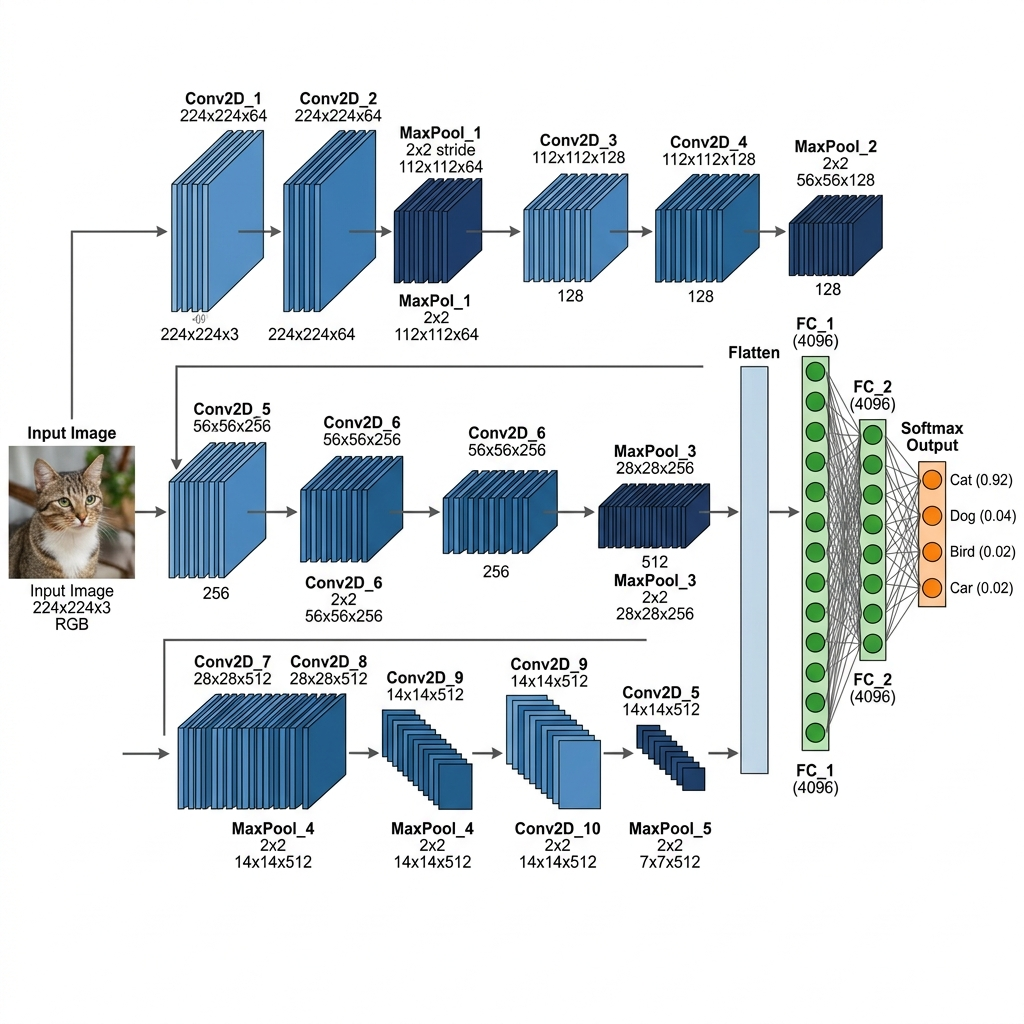
\includegraphics[width=0.9\textwidth]{docs/images/cnn_architecture.png}
\end{figure}

\subsection{Giới hạn của CNN trong nhận dạng bệnh lúa}
Mặc dù CNN đã chứng minh hiệu quả cao trong nhiều bài toán thị giác máy tính, song kiến trúc này mang những hạn chế cố hữu xuất phát từ chính thiết kế nền tảng của nó, đặc biệt bộc lộ rõ khi áp dụng vào bài toán phân tích hình thái bệnh lúa — một lĩnh vực đòi hỏi sự hiểu biết không gian tinh tế và khả năng diễn giải kết quả minh bạch.

\begin{enumerate}[leftmargin=1.5cm]
    \item \textbf{Trường thụ cảm cục bộ (Local Receptive Field):} Mỗi nơ-ron tích chập trong CNN chỉ xử lý một vùng không gian nhỏ của ảnh đầu vào, được giới hạn bởi kích thước bộ lọc (thường là 3×3 hoặc 5×5 pixel). Điều này có nghĩa là mô hình về bản chất chỉ "nhìn thấy" thông tin cục bộ tại mỗi bước xử lý. Để học được các phụ thuộc tầm xa (long-range dependencies) — ví dụ như mối liên hệ giữa vết bệnh xuất hiện ở đầu lá và các đốm hoại tử ở gốc lá — CNN buộc phải tích lũy thông tin qua rất nhiều lớp tích chập liên tiếp. Quá trình này không chỉ tốn kém về mặt tính toán mà còn kém hiệu quả, do thông tin toàn cục dễ bị suy giảm hoặc biến dạng khi truyền qua nhiều lớp biến đổi phi tuyến. Trong bài toán nhận dạng bệnh lúa, việc nắm bắt các mẫu phân bố không gian rộng — như sự lan rộng của đốm vân nâu hay hướng phát triển của vết cháy lá — là yếu tố quan trọng mà CNN xử lý chưa thực sự thỏa đáng.
    \item \textbf{Bất biến dịch chuyển:} CNN được thiết kế có chủ đích để đạt tính bất biến với phép dịch chuyển (translation invariance), tức là mô hình nhận dạng một đối tượng như nhau dù nó xuất hiện ở bất kỳ vị trí nào trong ảnh. Đây là ưu điểm trong nhiều bài toán phân loại ảnh tổng quát, nhưng lại trở thành hạn chế đáng kể trong phân tích bệnh lúa. Trên thực tế, vị trí tuyệt đối của vết bệnh trên lá mang thông tin chẩn đoán quan trọng: bệnh đạo ôn (blast) thường xuất hiện ở chóp lá hoặc cổ bông, bệnh khô vằn (sheath blight) tập trung ở bẹ lá phía dưới gần mặt nước, trong khi bệnh bạc lá (bacterial leaf blight) thường khởi phát từ mép lá. Khi CNN xóa bỏ thông tin vị trí thông qua các lớp pooling, những tín hiệu không gian có giá trị này bị mất đi, làm giảm khả năng phân biệt chính xác giữa các loại bệnh có hình thái vết bệnh tương đồng.
    \item \textbf{Phụ thuộc vào quy mô:} Kích thước vết bệnh trên lúa có thể dao động rất lớn tùy theo giai đoạn phát triển của bệnh, điều kiện môi trường và giống lúa — từ những đốm nhỏ vài milimet ở giai đoạn khởi phát đến các vùng hoại tử rộng hàng centimet ở giai đoạn bệnh nặng. CNN với các bộ lọc có kích thước cố định gặp khó khăn đáng kể khi cần nhận dạng cùng một loại bệnh ở các tỷ lệ khác nhau. Để khắc phục, người ta phải tích hợp các kỹ thuật bổ sung như multi-scale feature extraction hay Feature Pyramid Network (FPN) — tức là xây dựng các nhánh xử lý song song ở nhiều độ phân giải khác nhau rồi hợp nhất thông tin lại. Điều này làm tăng đáng kể độ phức tạp của kiến trúc, chi phí huấn luyện, cũng như khó khăn trong việc tinh chỉnh siêu tham số, trong khi hiệu quả đạt được vẫn chưa thực sự nhất quán trên mọi điều kiện thu thập ảnh thực địa.
    \item \textbf{Giải thích kém:} CNN về bản chất là một "hộp đen" (black box): mặc dù mô hình có thể đưa ra dự đoán với độ chính xác cao, nhưng quá trình ra quyết định bên trong — tại sao mô hình phân loại một mẫu bệnh cụ thể là đạo ôn thay vì đốm nâu — gần như không thể diễn giải một cách trực tiếp. Các kỹ thuật trực quan hóa như Grad-CAM hay saliency maps chỉ cung cấp được những gợi ý mờ nhạt về vùng ảnh mà mô hình "chú ý" đến, chứ chưa giải thích được cơ chế ra quyết định một cách thực sự tường minh. Đây là hạn chế đặc biệt nghiêm trọng trong các ứng dụng nông nghiệp và y tế thực tiễn, nơi người dùng cuối — như các kỹ sư nông nghiệp, nhà nghiên cứu bệnh cây, hay nông dân — cần hiểu được căn cứ của dự đoán để quyết định biện pháp xử lý phù hợp, đồng thời đặt ra yêu cầu về trách nhiệm giải trình (accountability) đối với hệ thống hỗ trợ quyết định.
\end{enumerate}

\section{Vision Transformer (ViT)}

\subsection{Từ xử lý ngôn ngữ tự nhiên (NLP) sang Thị giác máy tính}

Tiến trình phát triển của kiến trúc Transformer bắt đầu từ cột mốc quan trọng vào năm 2017, khi Vaswani cùng các cộng sự chính thức giới thiệu mô hình này nhằm giải quyết triệt để bài toán dịch máy trong lĩnh vực NLP. Khác biệt hoàn toàn với các kiến trúc truyền thống dựa trên tính hồi quy (recurrence) vốn xử lý dữ liệu theo tuần tự, Transformer đặt nền tảng trên cơ chế chú ý (attention), cho phép mô hình tập trung vào các phần quan trọng của dữ liệu đầu vào một cách linh hoạt và hiệu quả hơn. Đến năm 2020, một bước ngoặt mới đã xảy ra khi Dosovitskiy và nhóm nghiên cứu tại Google Brain thực hiện một thử nghiệm táo bạo: áp dụng trực tiếp kiến trúc Transformer thuần túy — vốn được thiết kế cho văn bản — vào dữ liệu hình ảnh, từ đó tạo ra mô hình Vision Transformer (ViT). Kết quả thực nghiệm cho thấy, khi được cung cấp một lượng dữ liệu tiền huấn luyện đủ lớn, ViT không chỉ đạt được hiệu năng ngang bằng mà còn có khả năng vượt trội hơn cả các mạng nơ-ron tích chập (CNN) tiêu chuẩn trên tập dữ liệu thử nghiệm ImageNet, mở ra một kỷ nguyên mới cho việc ứng dụng các kiến trúc dạng chuỗi vào bài toán thị giác.
\newpage
\subsection{Chia ảnh thành các Patch}
Thay vì xử lý từng pixel, ViT chia ảnh đầu vào $H \times W \times C$ thành $N$ patch (mảnh) không chồng lấp có kích thước $P \times P$:
\begin{equation}
    N = \frac{H \times W}{P^2}
    \label{eq:num_patches}
\end{equation}
Với ảnh $224 \times 224$ và $P = 16$: $N = \frac{224^2}{16^2} = 196$ patch. Mỗi patch được làm phẳng (flatten) thành vector 1D và chiếu tuyến tính vào không gian nhúng (embedding) chiều $D$:
\begin{equation}
    \mathbf{z}_i = \mathbf{E} \cdot \text{flatten}(\mathbf{x}_i^p) + \mathbf{e}_i^{pos}
    \label{eq:patch_embed}
\end{equation}
trong đó $\mathbf{E} \in \mathbb{R}^{D \times (P^2 \cdot C)}$ là ma trận chiếu học được, $\mathbf{e}_i^{pos}$ là mã hóa vị trí.

\subsection{Mã hóa vị trí (Positional Encoding)}
Khác biệt hoàn toàn với các mạng nơ-ron tích chập (CNN) — vốn sở hữu cấu trúc không gian tường minh nhờ vào đặc tính của các phép toán tích chập trên vùng lân cận — kiến trúc Transformer lại xử lý các phân mảnh hình ảnh (patches) như một chuỗi các phần tử độc lập và không có thứ tự sắp xếp tự thân. Do mô hình không thể tự nhận biết được vị trí tương đối giữa các mảnh ảnh, thông tin về tọa độ không gian bắt buộc phải được bổ sung thông qua kỹ thuật mã hóa vị trí học được (learned positional encoding). Cụ thể, các vector mã hóa này sẽ được cộng trực tiếp vào các vector biểu diễn phân mảnh (patch embedding) để giúp mô hình giữ lại được cấu trúc hình học của bức ảnh gốc. Đây là một điểm điều chỉnh quan trọng và khác biệt so với các mô hình Transformer trong lĩnh vực Xử lý ngôn ngữ tự nhiên (NLP), vốn thường sử dụng các hàm lượng giác sin/cos cố định để mã hóa vị trí của các từ trong văn bản. Thay vì dùng các giá trị toán học định sẵn, Vision Transformer cho phép mô hình tự học các vector vị trí này trong quá trình huấn luyện để tối ưu hóa khả năng nhận diện đặc trưng không gian.

\subsection{Token CLS và chuỗi đầu vào}
Một token đặc biệt $[\text{CLS}]$ được thêm vào đầu chuỗi, tương tự BERT trong NLP. Sau khi qua các lớp Transformer, đầu ra tương ứng với $[\text{CLS}]$ được dùng làm biểu diễn tổng thể của ảnh để phân loại:
\begin{equation}
    \mathbf{z}_0 = [\mathbf{x}_\text{class};\, \mathbf{z}_1;\, \mathbf{z}_2;\, \ldots;\, \mathbf{z}_N] + \mathbf{E}_{pos}
    \label{eq:cls_token}
\end{equation}
\newpage
\subsection{Cơ chế Multi-Head Self-Attention (MHSA)}
Đây là trái tim của ViT. Self-Attention cho phép mỗi patch "nhìn thấy" tất cả các patch khác và học trọng số quan tâm:

\textbf{Bước 1 --- Tính Q, K, V:} Mỗi token nhúng được chiếu thành ba vector:
\begin{equation}
    Q = \mathbf{z}W^Q, \quad K = \mathbf{z}W^K, \quad V = \mathbf{z}W^V
\end{equation}
trong đó $W^Q, W^K, W^V \in \mathbb{R}^{D \times d_k}$ là các ma trận trọng số học được.

\textbf{Bước 2 --- Tính điểm Attention:}
\begin{equation}
    \text{Attention}(Q, K, V) = \text{softmax}\!\left(\frac{QK^\top}{\sqrt{d_k}}\right)\!V
    \label{eq:attention}
\end{equation}
Hệ số $\frac{1}{\sqrt{d_k}}$ dùng để ổn định gradient khi $d_k$ lớn.

\textbf{Bước 3 --- Multi-Head:} Phép attention được thực hiện song song $h$ lần với các không gian chiếu khác nhau:
\begin{equation}
    \text{MultiHead}(Q,K,V) = \text{Concat}(\text{head}_1, \ldots, \text{head}_h)W^O
    \label{eq:multihead}
\end{equation}
\begin{equation}
    \text{head}_i = \text{Attention}(QW_i^Q, KW_i^K, VW_i^V)
\end{equation}
Với ViT-Base: $h = 12$ heads, $d_k = 64$, $D = 768$.

\subsection{Khối Transformer Encoder}
Mỗi khối Transformer Encoder gồm hai thành phần với kết nối tắt (skip connection) và chuẩn hóa lớp (Layer Normalization):
\begin{align}
    \mathbf{z}'_\ell &= \text{MHSA}(\text{LN}(\mathbf{z}_{\ell-1})) + \mathbf{z}_{\ell-1} \\
    \mathbf{z}_\ell  &= \text{MLP}(\text{LN}(\mathbf{z}'_\ell)) + \mathbf{z}'_\ell
\end{align}
trong đó MLP (Multi-Layer Perceptron) gồm hai lớp tuyến tính với hàm kích hoạt GELU:
\begin{equation}
    \text{GELU}(x) = x \cdot \Phi(x)
\end{equation}
với $\Phi(x)$ là hàm phân phối tích lũy của phân phối chuẩn.

\begin{figure}[H]{Kiến trúc Vision Transformer (ViT): ảnh được chia thành các patch, nhúng vào không gian embedding, xử lý qua $L$ khối Transformer Encoder và phân loại qua MLP head.}
    \centering
    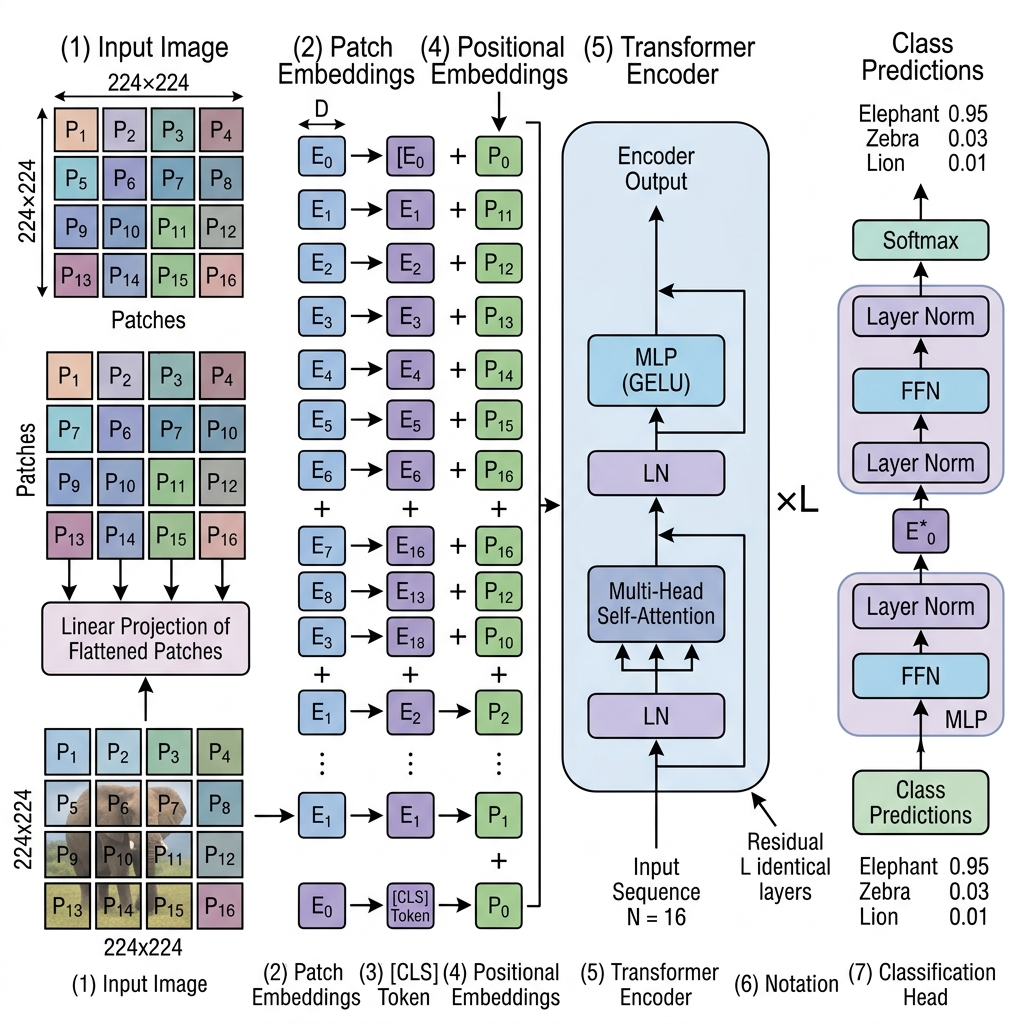
\includegraphics[width=0.9\textwidth]{docs/images/vit_architecture.png}
\end{figure}
\newpage
\subsection{Đầu phân loại và tinh chỉnh}
Sau $L$ khối Transformer, đầu ra của token $[\text{CLS}]$ đi qua một lớp MLP phân loại:
\begin{equation}
    \hat{y} = \text{softmax}(W_\text{cls} \cdot \text{LN}(\mathbf{z}_L^0) + b_\text{cls})
\end{equation}
Mô hình được tiền huấn luyện trên ImageNet-21k (14 triệu ảnh, 21,843 lớp) rồi tinh chỉnh (fine-tune) trên tập dữ liệu lá lúa \texttt{prithivMLmods/Rice-Leaf-Disease} với 4 lớp đầu ra.

\begin{table}[H]{So sánh thông số của các biến thể ViT}
\centering
\begin{tabular}{lcccc}
\toprule
\textbf{Biến thể} & \textbf{Layers (L)} & \textbf{Hidden size (D)} & \textbf{Heads (h)} & \textbf{Params} \\
\midrule
ViT-Tiny  & 12 & 192  & 3  & 5.7M \\
ViT-Small & 12 & 384  & 6  & 22M \\
ViT-Base  & 12 & 768  & 12 & 86M \\
ViT-Large & 24 & 1024 & 16 & 307M \\
ViT-Huge  & 32 & 1280 & 16 & 632M \\
\bottomrule
\end{tabular}
\end{table}

\section{Mô hình ngôn ngữ lớn (LLM) và Gemini}

\subsection{Kiến trúc Transformer Decoder}
Trong khi ViT (Vision Transformer) sử dụng kiến trúc Transformer Encoder — nơi mỗi token có thể chú ý đến toàn bộ các token khác trong chuỗi theo cả hai chiều — các mô hình ngôn ngữ lớn thế hệ mới như GPT (OpenAI) hay Gemini (Google DeepMind) lại áp dụng kiến trúc Transformer Decoder với cơ chế causal self-attention (hay còn gọi là masked self-attention). Trong cơ chế này, mỗi token chỉ được phép chú ý đến chính nó và các token đứng trước đó trong chuỗi, hoàn toàn không có quyền truy cập vào các token phía sau. Thiết kế này đảm bảo tính nhân quả trong quá trình sinh văn bản: mô hình không thể "nhìn trước" tương lai khi đang dự đoán hiện tại.\\
\indent Nhiệm vụ huấn luyện cốt lõi của các mô hình này là dự đoán token tiếp theo trong chuỗi (next-token prediction) — tức là, cho trước một đoạn văn bản, mô hình học cách ước tính token nào có xác suất xuất hiện cao nhất ở vị trí kế tiếp. Tuy đây là một mục tiêu huấn luyện đơn giản, nhưng khi được áp dụng lặp đi lặp lại trên một kho ngữ liệu khổng lồ lên đến hàng nghìn tỷ token văn bản — bao gồm sách, bài báo, trang web, mã nguồn và nhiều dạng nội dung khác — mô hình buộc phải ngầm học các quy luật ngữ pháp, cấu trúc lập luận, kiến thức thực tế và thậm chí cả khả năng suy luận nhiều bước. Đây chính là cơ chế mà qua đó các mô hình ngôn ngữ lớn hấp thụ tri thức một cách rộng rãi và sâu sắc từ thế giới văn bản.

\subsection{Mô hình Gemini của Google DeepMind}
Gemini được biết đến là một họ mô hình đa phương thức tiên tiến do Google DeepMind nghiên cứu và phát triển, sở hữu khả năng vượt trội trong việc tiếp nhận và xử lý đồng thời nhiều loại dữ liệu đầu vào khác nhau bao gồm văn bản, hình ảnh, âm thanh và video chỉ trong cùng một lời nhắc (prompt) [5]. Trong phạm vi triển khai của đề tài, hệ thống đã lựa chọn sử dụng phiên bản Gemini 2.5 Flash. Đây là phiên bản được tối ưu hóa để đạt được sự cân bằng lý tưởng giữa tốc độ xử lý và độ chính xác của dữ liệu đầu ra, hoàn toàn phù hợp với các bài toán thực tế yêu cầu phản hồi trong một khoảng thời gian chờ đợi chấp nhận được.

Lý do chính yếu cho việc ưu tiên lựa chọn Gemini 2.5 Flash thay vì các phiên bản có cấu trúc phức tạp và mạnh mẽ hơn như Gemini Pro nằm ở vấn đề độ trễ (latency). Các kết quả thực nghiệm thực tế cho thấy, phiên bản Flash có khả năng trả về kết quả nhanh chóng trong khoảng $\approx$ 5–8 giây; trong khi đó, phiên bản Pro có thể kéo dài thời gian phản hồi lên tới 15–20 giây—một mức độ trễ được đánh giá là quá lâu và không đáp ứng được yêu cầu về trải nghiệm người dùng thực tế. Bên cạnh đó, tham số nhiệt độ sinh văn bản ($T$) cũng được thiết lập chuyên biệt cho từng tác vụ: mức $T$ được đặt ở 0.2 đối với Morphology Agent nhằm đảm bảo các mô tả hình thái mang tính khách quan và chính xác, trong khi mức $T$ được nâng lên 0.4 đối với Coordinator Agent để tạo ra các báo cáo có sự linh hoạt và uyển chuyển hơn về mặt ngôn ngữ.

Tuy nhiên, hệ thống vẫn tồn tại một số hạn chế nhất định cần được lưu ý như việc sử dụng Gemini API bắt buộc phải có kết nối Internet ổn định và bị ràng buộc bởi giới hạn số lượng lượt gọi theo định mức của gói miễn phí. Hiện tại, hệ thống vẫn chưa có cơ chế tự động xử lý trong các tình huống API bị quá tải hoặc xảy ra gián đoạn kết nối—đây được xác định là những điểm trọng yếu cần được nghiên cứu và cải thiện trong các phiên bản nâng cấp tiếp theo.

\section{RAG và ChromaDB}

\subsection{Vấn đề Hallucination của LLM}
Mặc dù các mô hình ngôn ngữ lớn (LLM) hiện nay sở hữu khả năng xử lý và tạo lập ngôn ngữ vô cùng phi thường, chúng vẫn tồn tại một hạn chế cố hữu là xu hướng xảy ra hiện tượng "ảo giác" (hallucination). Đây là trạng thái mà mô hình tự bịa đặt ra những thông tin nghe có vẻ rất hợp lý và thuyết phục về mặt ngôn từ, nhưng về bản chất lại hoàn toàn sai lệch so với thực tế. Trong bối cảnh chuyên biệt như ngành nông nghiệp, những sai sót này không chỉ dừng lại ở mức độ thông tin thuần túy; chẳng hạn, một khuyến nghị sai lệch về liều lượng sử dụng thuốc bảo vệ thực vật có thể trực tiếp dẫn đến những thiệt hại nghiêm trọng về kinh tế và cây trồng. 
\newpage Để giải quyết vấn đề này, RAG (Retrieval-Augmented Generation) được ứng dụng như một giải pháp chủ chốt nhằm kiểm soát và giảm thiểu hiện tượng "ảo giác". Bằng cách truy xuất và cung cấp các ngữ cảnh thực tế từ một kho tri thức đã được kiểm chứng và xác thực độ tin cậy, RAG buộc mô hình phải dựa trên các căn cứ xác thực thay vì tự suy diễn, từ đó đảm bảo tính chính xác cho các phản hồi đầu ra.

\subsection{Kiến trúc RAG}
RAG bổ sung một bước truy xuất thông tin vào quy trình sinh văn bản, gồm hai giai đoạn:

\textbf{Giai đoạn Lập chỉ mục (Indexing --- offline):}
\begin{enumerate}[leftmargin=1.5cm]
    \item \textbf{Nạp tài liệu:} Các tài liệu về bệnh học cây lúa, phác đồ điều trị.
    \item \textbf{Phân đoạn (Chunking):} Chia tài liệu thành các đoạn (chunk) nhỏ.
    \item \textbf{Nhúng (Embedding):} Chuyển đổi mỗi chunk thành vector số học chiều cao bằng mô hình embedding.
    \item \textbf{Lưu trữ:} Lưu các vector vào cơ sở dữ liệu vector (ChromaDB).
\end{enumerate}

\textbf{Giai đoạn Truy vấn (Query --- online):}
\begin{enumerate}[leftmargin=1.5cm]
    \item Câu hỏi người dùng được nhúng thành vector bằng cùng mô hình embedding.
    \item Tìm kiếm tương đồng vector trong ChromaDB để lấy $k$ tài liệu liên quan nhất.
    \item Ghép tài liệu truy xuất + câu hỏi gốc thành một lời nhắc (prompt) cho LLM.
    \item LLM sinh câu trả lời dựa trên ngữ cảnh thực tế được cung cấp.
\end{enumerate}

\begin{figure}[H]{Kiến trúc pipeline RAG hai giai đoạn: Indexing (lập chỉ mục offline) và Query (truy vấn online). ChromaDB đóng vai trò là kho lưu trữ vector trung tâm.}
    \centering
    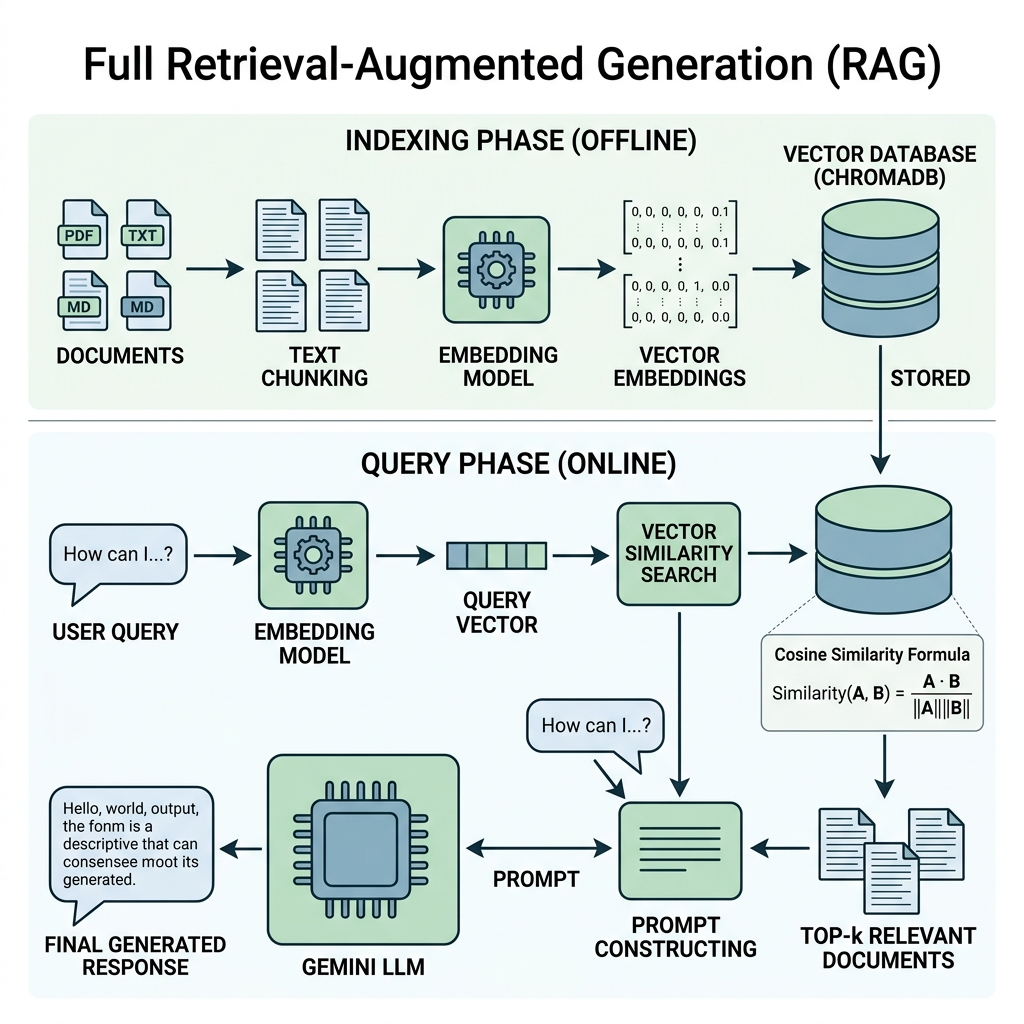
\includegraphics[width=0.8\textwidth]{docs/images/rag_pipeline.png}
\end{figure}

\subsection{Độ tương đồng Cosine}
Phép đo quan trọng nhất trong tìm kiếm vector là độ tương đồng cosine --- đo góc giữa hai vector thay vì khoảng cách Euclidean, do đó không bị ảnh hưởng bởi độ dài vector:
\begin{equation}
    \text{sim}(\mathbf{A}, \mathbf{B}) = \cos(\theta) = \frac{\mathbf{A} \cdot \mathbf{B}}{\|\mathbf{A}\|\|\mathbf{B}\|} = \frac{\displaystyle\sum_{i=1}^{n} A_i B_i}{\sqrt{\displaystyle\sum_{i=1}^{n}A_i^2} \cdot \sqrt{\displaystyle\sum_{i=1}^{n}B_i^2}}
    \label{eq:cosine}
\end{equation}
Giá trị $\text{sim} \in [-1, 1]$; trong không gian embedding thực tế, $\text{sim} \in [0, 1]$. Hệ thống chỉ truy xuất tài liệu với $\text{sim} > 0.82$ để đảm bảo độ liên quan.

\subsection{ChromaDB}
ChromaDB đóng vai trò là cơ sở dữ liệu vector mã nguồn mở (phát hành dưới giấy phép Apache 2.0), được thiết kế với kiến trúc tối ưu chuyên biệt cho các tác vụ của quy trình Thế năng tăng cường truy xuất (RAG). Một trong những đặc điểm nổi bật nhất của ChromaDB là khả năng lưu trữ cục bộ trực tiếp trên ổ đĩa (persistent storage), giúp dữ liệu được duy trì bền vững mà không nhất thiết phải thiết lập hay quản lý một hệ thống server riêng biệt, từ đó đơn giản hóa cấu hình hệ thống. Trong quá trình triển khai, ChromaDB thể hiện khả năng tương thích cao thông qua việc tích hợp trực tiếp với khung làm việc LangChain thông qua thư viện langchain-community, giúp quá trình kết nối và điều phối dữ liệu trở nên liền mạch.

Về mặt chức năng, hệ thống hỗ trợ cơ chế lọc theo siêu dữ liệu (metadata filtering), cho phép người dùng thực hiện các truy vấn tinh lọc dựa trên các tiêu chí cụ thể như loại bệnh lý hoặc nguồn tài liệu nguồn, giúp thu hẹp phạm vi tìm kiếm và tăng độ chính xác của thông tin truy xuất. Để đảm bảo hiệu suất vận hành, ChromaDB sử dụng thuật toán chỉ mục HNSW (Hierarchical Navigable Small World). Đây là một thuật toán tiên tiến cho phép thực hiện các phép tìm kiếm láng giềng gần đúng (Approximate Nearest Neighbor) một cách cực kỳ hiệu quả, duy trì tốc độ phản hồi nhanh ngay cả khi phải xử lý trên các tập dữ liệu có quy mô lớn.

\section{Lý thuyết AI Agent}

\subsection{Định nghĩa AI Agent}

AI Agent (Tác nhân trí tuệ nhân tạo) là một hệ thống có khả năng hoạt động một cách tự chủ để hoàn thành các nhiệm vụ được giao, thông qua việc thiết kế các workflow (luồng công việc) sử dụng các công cụ có sẵn \cite{ibm2025}. Một AI Agent thường không chỉ thực hiện xử lý ngôn ngữ tự nhiên (NLP), mà còn có khả năng ra quyết định, giải quyết vấn đề, tương tác với môi trường bên ngoài và thực hiện các hành động liên quan để đạt được mục tiêu.

Tại lõi của AI Agent thường là một mô hình ngôn ngữ lớn (LLM). Những mô hình này được sử dụng để hiểu yêu cầu của người dùng, tạo ra các bước xử lý và quyết định thời điểm gọi đến các công cụ bên ngoài (tool calling) khi cần thiết. Trong nhiều tài liệu, AI Agent còn được gọi là ``LLM agents'' do vai trò trung tâm của LLM trong kiến trúc của nó \cite{sumers2023}.

Cần phân biệt AI Agent với các khái niệm liên quan: một \textbf{AI Assistant} (trợ lý AI) phản hồi trực tiếp theo từng yêu cầu của người dùng và dừng lại khi hoàn thành câu trả lời, trong khi AI Agent có khả năng tự lập kế hoạch, tự đặt ra các nhiệm vụ phụ và tiếp tục hành động mà không cần giám sát liên tục từ con người. Ranh giới quan trọng nhất là \textbf{tính tự chủ}: Agent có thể quyết định \emph{khi nào} và \emph{bằng công cụ nào} để hoàn thành mục tiêu, còn Assistant chỉ đưa ra kết quả theo yêu cầu tức thời.

\subsection{Các đặc điểm nổi bật của AI Agent}

Năm đặc điểm chính phân biệt AI Agent với các hệ thống AI truyền thống \cite{sumers2023}:

\textbf{Tự chủ (Autonomy):} AI Agent có khả năng đưa ra quyết định mà không cần sự can thiệp liên tục từ người dùng trong từng bước. Nó có thể tự tạo các nhiệm vụ phụ (subtasks) để hoàn thiện mục tiêu tổng thể. Đây là đặc điểm cốt lõi nhất phân biệt Agent với một hàm xử lý thông thường.

\textbf{Kết hợp công cụ bên ngoài (Tool-calling):} Khi nội tại của mô hình không đủ kiến thức hoặc khả năng, AI Agent có thể gọi các API, truy vấn cơ sở dữ liệu, sử dụng các mô-đun chuyên biệt hoặc thậm chí tương tác với các Agent khác để thu thập thông tin hoặc thực hiện tác vụ. Nhờ vậy, nó có thể cập nhật thông tin thời gian thực, xử lý dữ liệu mới và mở rộng khả năng giải quyết các nhiệm vụ phức tạp. Trong hệ thống của đề tài, mỗi Agent chính là một ``công cụ'' mà Coordinator Agent gọi đến theo trình tự.

\textbf{Bộ nhớ và khả năng học từ tương tác (Memory \& Reflection):} AI Agent có khả năng lưu giữ thông tin từ các tương tác trước --- tức là có ``nhớ'' --- để tinh chỉnh cách hoạt động, phản hồi và đáp ứng theo sở thích người dùng. Nó học từ phản hồi của người dùng hoặc từ các Agent khác, sử dụng dữ liệu đó để tự điều chỉnh và cải thiện dần theo thời gian. Trong hệ thống hiện tại, bộ nhớ được thể hiện thông qua ChromaDB lưu trữ tri thức bệnh học bền vững qua các phiên làm việc.

\textbf{Khả năng lập kế hoạch \& lý luận (Planning \& Reasoning):} AI Agent phân tích mục tiêu cấp cao, phân rã thành các bước con, đưa ra kế hoạch hành động để đạt mục tiêu. Trong quá trình thực thi, nó cũng thực hiện reasoning (lý luận) để đánh giá lại kế hoạch, tự hiệu chỉnh và chọn phương án tối ưu dựa trên thông tin mới thu thập được. Coordinator Agent trong đề tài thực hiện vai trò này bằng cách quyết định thứ tự gọi các Agent phụ và cách tổng hợp kết quả cuối cùng.

\textbf{Khả năng thích ứng và mở rộng (Adaptivity \& Scalability):} Nhờ học hỏi và phản hồi liên tục, AI Agent có thể thích ứng với đặc điểm riêng của người dùng hoặc ngữ cảnh cụ thể. Khi được triển khai trong kiến trúc đa tác nhân (multi-agent), nó có thể phối hợp với các Agent khác để mở rộng khả năng, tăng hiệu quả và tính linh hoạt. Kiến trúc của đề tài được thiết kế để thêm một Agent mới chỉ cần viết một lớp Python và đăng ký vào Coordinator, không cần thay đổi các Agent hiện có.

\subsection{Phân loại AI Agent}

Dựa trên mức độ phức tạp và khả năng ra quyết định, AI Agent được phân thành năm loại chính từ đơn giản đến phức tạp \cite{sumers2023}:

\textbf{Simple Reflex Agent (Tác nhân phản xạ đơn giản):} Là dạng kiến trúc cơ bản nhất, hoạt động hoàn toàn dựa trên sự phản ứng trực tiếp với trạng thái hiện tại của môi trường theo các quy tắc điều kiện--hành động được định sẵn. Tác nhân chỉ xem xét những gì nó cảm nhận được ngay tại thời điểm hiện tại để ra quyết định, bỏ qua kinh nghiệm trong quá khứ cũng như không tính đến hệ quả tương lai. Ưu điểm là tốc độ và độ đơn giản; hạn chế là không xử lý được môi trường thay đổi hoặc tình huống ngoại lệ.

\textbf{Model-Based Reflex Agent (Tác nhân phản xạ dựa trên mô hình):} Phiên bản nâng cao tích hợp thêm một mô hình nội tại về thế giới (world model), cho phép lưu trữ và theo dõi trạng thái môi trường qua thời gian, hiểu được cách các hành động trong quá khứ đã ảnh hưởng đến trạng thái hiện tại. Nhờ đó, tác nhân có thể ra quyết định chính xác hơn ngay cả khi không thể quan sát đầy đủ môi trường tức thời.

\textbf{Goal-Based Agent (Tác nhân dựa trên mục tiêu):} Không chỉ phản ứng với trạng thái hiện tại mà còn lập kế hoạch hành động hướng đến một mục tiêu cụ thể. Tác nhân đánh giá nhiều chuỗi hành động khác nhau và chọn chuỗi dẫn đến trạng thái mong muốn, thường sử dụng các thuật toán tìm kiếm và lập kế hoạch. Đây là nền tảng lý thuyết cho Coordinator Agent trong đề tài: mục tiêu là báo cáo chẩn đoán hoàn chỉnh, kế hoạch là gọi 4 Agent phụ theo đúng thứ tự.

\textbf{Utility-Based Agent (Tác nhân dựa trên độ hữu dụng):} Mở rộng từ Goal-Based bằng cách không chỉ tìm kiếm trạng thái mục tiêu mà còn tối ưu hóa chất lượng của kết quả đạt được thông qua hàm độ hữu dụng (utility function). Khi có nhiều cách đạt mục tiêu, tác nhân chọn phương án tối ưu nhất theo tiêu chí đã xác định (ví dụ: nhanh nhất, ít tốn kém nhất, độ chính xác cao nhất).

\textbf{Learning Agent (Tác nhân học):} Đây là loại Agent tiên tiến nhất, có thể cải thiện hiệu năng theo thời gian thông qua kinh nghiệm tích lũy. Learning Agent gồm bốn thành phần: (1) phần tử học (learning element) để cải thiện từ phản hồi, (2) phần tử thực thi (performance element) để đưa ra hành động, (3) phần tử phê bình (critic) để đánh giá kết quả, và (4) phần tử tạo vấn đề (problem generator) để khám phá trạng thái mới. Đây là hướng phát triển tương lai cho hệ thống: nếu có cơ chế thu thập phản hồi từ nông dân, hệ thống có thể học và tinh chỉnh dần theo thời gian.

\subsection{So sánh AI Agent và AI Assistant}

Một điểm dễ gây nhầm lẫn là sự khác biệt giữa AI Agent và AI Assistant. Bảng~\ref{tab:agent_vs_assistant} tóm tắt các khác biệt chính:

\begin{table}[H]{So sánh AI Agent và AI Assistant}
\label{tab:agent_vs_assistant}
\centering
\begin{tabularx}{\textwidth}{>{\bfseries}p{3.2cm} X X}
\toprule
\textbf{Tiêu chí} & \textbf{AI Assistant} & \textbf{AI Agent} \\
\midrule
Tính tự chủ & Thấp --- phản hồi theo yêu cầu tức thời & Cao --- tự lập kế hoạch và hành động \\[4pt]
Trí nhớ & Ngắn hạn, trong cửa sổ ngữ cảnh & Bền vững, lưu trữ qua các phiên \\[4pt]
Phạm vi công cụ & Hạn chế theo API được lập trình sẵn & Kết nối sâu với hệ thống bên ngoài \\[4pt]
Vai trò hành động & Đề xuất, con người quyết định & Tự thực hiện hành động đầu cuối \\[4pt]
Phân rã nhiệm vụ & Không tự phân rã & Tự tạo subtask để đạt mục tiêu \\[4pt]
Phối hợp & Độc lập & Phối hợp với Agent khác trong hệ sinh thái \\
\bottomrule
\end{tabularx}
\end{table}

Phản hồi của AI Assistant là kết quả trực tiếp của yêu cầu hiện tại, không có khả năng tiếp tục hành động khi được hướng dẫn thêm. Trong khi đó, AI Agent thể hiện tính tự chủ cao hơn. Sau khi nhận mục tiêu ban đầu, chúng có thể tự phân tích, suy luận, lập kế hoạch và hành động mà không cần sự giám sát liên tục của con người. AI Agent còn có thể tự đặt ra nhiệm vụ phụ, điều chỉnh chiến lược khi điều kiện thay đổi và hoàn thành mục tiêu theo cách tối ưu nhất \cite{ibm2025}.

Trong đề tài này, hệ thống được thiết kế theo mô hình \textbf{Goal-Based Multi-Agent}: mỗi Agent phụ (Preprocessing, Classification, Morphology, Retrieval) hoạt động như một Simple Reflex Agent chuyên biệt, còn Coordinator Agent đóng vai trò Goal-Based Agent điều phối toàn bộ quy trình hướng đến mục tiêu là báo cáo chẩn đoán cuối cùng.

\subsection{Hệ thống Đa Tác Nhân (Multi-Agent System)}

Một Hệ thống Đa Tác Nhân (MAS --- Multi-Agent System) là tập hợp nhiều Agent tự trị cùng hoạt động và phối hợp trong một môi trường chung để giải quyết các bài toán phức tạp mà một Agent đơn lẻ không thể xử lý hiệu quả. Mỗi Agent trong hệ thống có thể có mục tiêu riêng, nhưng hành động của chúng được điều phối để đạt được mục tiêu chung của toàn hệ thống.

Ưu điểm của kiến trúc MAS so với một Agent đơn hoặc pipeline đơn thuần:

\begin{itemize}[leftmargin=1.5cm]
    \item \textbf{Phân chia trách nhiệm (Separation of Concerns):} Mỗi Agent chuyên trách một nhiệm vụ cụ thể, giúp code dễ bảo trì và kiểm thử độc lập.
    \item \textbf{Khả năng mở rộng:} Thêm năng lực mới vào hệ thống chỉ cần thêm Agent mới mà không cần thay đổi các Agent hiện có.
    \item \textbf{Chịu lỗi tốt hơn (Fault Tolerance):} Nếu một Agent gặp lỗi, Coordinator có thể xử lý ngoại lệ mà không làm sập toàn bộ hệ thống.
    \item \textbf{Phối hợp tự trị:} Các Agent có thể phối hợp theo luồng điều phối (orchestration) hoặc tự thương lượng (negotiation) tùy theo kiến trúc.
\end{itemize}

\subsection{Mô hình phối hợp trong hệ thống}
Hệ thống sử dụng mô hình phối hợp \textbf{Orchestrated Sequential}: Coordinator Agent đóng vai trò nhạc trưởng, điều phối luồng thực thi tuần tự (preprocessing $\rightarrow$ classification $\rightarrow$ morphology $\rightarrow$ retrieval $\rightarrow$ report). Mô hình này được chọn thay vì song song hoàn toàn vì mỗi bước phụ thuộc vào đầu ra của bước trước: Classification Agent cần ảnh đã tiền xử lý; Morphology Agent cần biết nhãn bệnh để định hướng phân tích; Coordinator Agent cần đủ bốn kết quả để tổng hợp.

Một điểm thiết kế quan trọng là cơ chế \textbf{callback theo dõi tiến trình}: thay vì đợi toàn bộ pipeline chạy xong rồi trả kết quả, Coordinator gọi hàm \texttt{progress\_callback(msg)} sau mỗi bước. Giao diện Streamlit lắng nghe callback này và cập nhật thẻ trạng thái Agent ngay lập tức, tạo cảm giác đáp ứng nhanh dù tổng thời gian xử lý vẫn có thể mất $\sim$15 giây.

So sánh với phương án pipeline đơn giản (hàm gọi hàm theo thứ tự cứng), kiến trúc Agent mang lại hai lợi thế thực tế: (1) dễ thay thế từng Agent mà không ảnh hưởng các Agent khác --- ví dụ thay Gemini bằng một LLM khác chỉ cần sửa file \texttt{morphology.py}; (2) dễ kiểm thử độc lập từng Agent bằng unit test mà không cần chạy cả hệ thống.
\chapter{Thiết kế và Kiến trúc Hệ thống Multi-Agent}

\section{Kiến trúc tổng thể}

\subsection{Định hướng thiết kế}
Khi bắt đầu thiết kế hệ thống, tác giả đặt ra một câu hỏi thực tế: nếu cần thêm khả năng phát hiện một loại bệnh mới trong tương lai, cần sửa bao nhiêu chỗ trong code? Câu trả lời dẫn đến việc lựa chọn kiến trúc đa tác nhân theo nguyên tắc \textbf{Separation of Concerns} --- mỗi Agent chịu trách nhiệm duy nhất cho một nhiệm vụ và không phụ thuộc trực tiếp vào Agent khác. Nhờ đó, để thêm một Agent mới (ví dụ Agent kiểm tra chất lượng ảnh đầu vào), chỉ cần viết thêm một lớp Python và đăng ký vào Coordinator.

Kiến trúc ba tầng được áp dụng:
\begin{itemize}[leftmargin=1.5cm]
    \item \textbf{Tầng giao diện:} Streamlit UI --- nơi người dùng tương tác trực tiếp.
    \item \textbf{Tầng xử lý:} FastAPI Backend + Agent Pipeline --- điều phối toàn bộ logic nghiệp vụ.
    \item \textbf{Tầng dữ liệu:} ChromaDB Vector Store + trọng số mô hình ViT.
\end{itemize}

\subsection{Luồng xử lý dữ liệu end-to-end}
Kết nối giữa giao diện Streamlit và hệ thống Agent được thực hiện qua mô-đun \texttt{src/core/workflow.py} --- một lớp trung gian (bridge) được thiết kế để tách biệt logic UI và logic nghiệp vụ. Lý do dùng bridge thay vì gọi trực tiếp: Streamlit và FastAPI có chu kỳ sống khác nhau, và trong tương lai nếu muốn thay Streamlit bằng một frontend khác (React, Flutter), chỉ cần viết lại phần gọi bridge mà không đụng vào Agent.

Luồng dữ liệu đầy đủ diễn ra như sau:
\begin{enumerate}[leftmargin=1.5cm]
    \item Người dùng tải ảnh lá lúa lên giao diện Streamlit (JPG/PNG/WebP).
    \item Streamlit gọi hàm \texttt{run\_diagnosis(image, callback)} qua workflow bridge.
    \item \texttt{CoordinatorAgent.run()} nhận ảnh và \texttt{callback}, lần lượt gọi 4 Agent theo thứ tự, gọi \texttt{callback(trạng thái)} sau mỗi bước.
    \item Kết quả trả về là một từ điển Python gồm 5 khóa: \texttt{disease\_label}, \texttt{confidence}, \texttt{morphology\_analysis}, \texttt{knowledge\_info}, \texttt{final\_report}.
    \item Streamlit đọc từng khóa và hiển thị theo bố cục đã thiết kế.
\end{enumerate}

\begin{figure}[H]{Sơ đồ kiến trúc chi tiết hệ thống Đa Tác Vụ, thể hiện mối quan hệ giữa các Agent, API và cơ sở dữ liệu.}
    \centering
    \includegraphics[width=\textwidth]{docs/images/leaf.drawio.png}
\end{figure}

\section{Thiết kế chi tiết từng Agent}
\subsection{Preprocessing Agent}
\textbf{Chức năng:} Chuẩn hóa ảnh đầu vào, tách nền và tăng cường độ tương phản.

\textbf{Input:} Đối tượng \texttt{PIL.Image} bất kỳ kích thước, bất kỳ định dạng.

\textbf{Output:} Đối tượng \texttt{PIL.Image} chuẩn hóa $224 \times 224$ RGB.

\textbf{Thuật toán xử lý:}
\begin{enumerate}[leftmargin=1.5cm]
    \item \textbf{Tách nền:} Thư viện \texttt{rembg} sử dụng mô hình U-Net thu nhỏ (IS-Net, kích thước $\sim$170MB) được huấn luyện trên tập dữ liệu lớn để phân vùng đối tượng chính. Đầu ra là ảnh RGBA với kênh alpha là mask tách nền. Vùng nền alpha $< 127$ được thay bằng nền trắng $(255, 255, 255)$.
    \item \textbf{Tăng cường tương phản:} Dùng \texttt{PIL.ImageEnhance.Contrast} với hệ số $1.2$ ($+20\%$) giúp làm nổi bật các vết bệnh.
    \item \textbf{Resampling:} Resize về $224 \times 224$ bằng thuật toán Lanczos cho chất lượng tốt nhất khi thu nhỏ ảnh.
\end{enumerate}
\newpage
\begin{lstlisting}[language=Python, caption={Preprocessing Agent --- xử lý ảnh đầu vào}, label={lst:preprocessing}]
class PreprocessingAgent:
    def process(self, image: Image.Image) -> Image.Image:
        # 1. Tach nen bang rembg (U-Net)
        image_no_bg = remove(image)

        # 2. Chuyen RGBA -> RGB voi nen trang
        if image_no_bg.mode in ('RGBA', 'LA'):
            background = Image.new('RGB', image_no_bg.size, (255, 255, 255))
            background.paste(image_no_bg, mask=image_no_bg.split()[3])
            image_no_bg = background

        # 3. Tang cuong tuong phan +20%
        enhancer = ImageEnhance.Contrast(image_no_bg)
        image_enhanced = enhancer.enhance(1.2)

        # 4. Resize 224x224 Lanczos
        return image_enhanced.resize((224, 224), Image.Resampling.LANCZOS)
\end{lstlisting}

\subsection{Classification Agent}
\textbf{Chức năng:} Phân loại bệnh lúa từ ảnh đã tiền xử lý.

\textbf{Mô hình:} \texttt{prithivMLmods/Rice-Leaf-Disease} trên Hugging Face --- ViT-Base được fine-tune trên tập dữ liệu lá lúa với 4 nhãn: Blast, Blight, Brown Spot, Tungro.

\textbf{Quy trình suy luận:}
\begin{enumerate}[leftmargin=1.5cm]
    \item \textbf{Tiền xử lý ảnh:} \texttt{AutoImageProcessor} chuẩn hóa pixel về $[-1, 1]$, chuyển sang tensor PyTorch.
    \item \textbf{Suy luận:} Đưa tensor qua mô hình ViT trong chế độ \texttt{torch.no\_grad()} để tiết kiệm bộ nhớ.
    \item \textbf{Tính xác suất:} Áp dụng Softmax lên vector logits 4 chiều:
    \begin{equation}
        P(y_i | \mathbf{x}) = \frac{e^{z_i}}{\displaystyle\sum_{j=1}^{4} e^{z_j}}
        \label{eq:softmax}
    \end{equation}
    \item \textbf{Đầu ra:} Từ điển gồm nhãn dự đoán, độ tin cậy (\%), và phân phối xác suất toàn bộ 4 lớp.
\end{enumerate}

\begin{table}[H]{Thông số kỹ thuật của Classification Agent}
\centering
\begin{tabular}{lp{9cm}}
\toprule
\textbf{Thông số} & \textbf{Giá trị} \\
\midrule
Mô hình cơ sở & ViT-Base/16 (tiền huấn luyện ImageNet-21k) \\
Tập dữ liệu fine-tune & prithivMLmods/Rice-Leaf-Disease \\
Kích thước đầu vào & $224 \times 224 \times 3$ \\
Số lớp đầu ra & 4 (Blast, Blight, Brown Spot, Tungro) \\
Framework & PyTorch + HuggingFace Transformers \\
Thiết bị & CPU (tự động phát hiện GPU nếu có) \\
Kích thước mô hình & $\sim$330MB \\
Thời gian suy luận & $\sim$0.8s (CPU) \\
\bottomrule
\end{tabular}
\end{table}

\subsection{Morphology Agent}
\textbf{Chức năng:} Phân tích hình thái học của lá lúa bằng mô hình đa phương thức Gemini Vision.

\textbf{Chiến lược Prompt Engineering:} Agent sử dụng một lời nhắc có cấu trúc yêu cầu Gemini mô tả ba khía cạnh: (1) màu sắc vết bệnh, (2) hình dạng và kích thước, (3) phân bố trên lá, đồng thời đối chiếu với nhãn bệnh đã được Classification Agent xác định.

\textbf{Xử lý ảnh cho Gemini:} Ảnh PIL được mã hóa Base64 và nhúng trực tiếp vào nội dung HumanMessage theo chuẩn data URI:
\begin{equation}
    \text{Image URI} = \texttt{data:image/png;base64,} + \text{Base64}(\text{PNG bytes})
\end{equation}

\textbf{Tại sao không chỉ dùng ViT?} ViT cho nhãn phân loại nhưng không giải thích. Morphology Agent cung cấp tính giải thích được (explainability) --- nông dân hiểu tại sao hệ thống kết luận như vậy và có thể kiểm chứng bằng mắt thường.

\subsection{Retrieval Agent}
\textbf{Chức năng:} Truy xuất thông tin bệnh học chính xác từ ChromaDB.

\textbf{Cơ sở tri thức:} Bốn tài liệu tương ứng bốn loại bệnh, mỗi tài liệu chứa: tác nhân gây bệnh, đặc điểm nhận dạng, điều kiện phát triển, biện pháp phòng ngừa và điều trị.

\textbf{Mô hình Embedding:} \texttt{models/gemini-embedding-001} --- tạo ra vector nhúng 768 chiều cho mỗi đoạn tài liệu.

\textbf{Tìm kiếm:} \texttt{vectorstore.similarity\_search(disease\_query, k=1)} tìm tài liệu gần nhất theo cosine similarity.

\begin{table}[H]{Cấu trúc tài liệu trong ChromaDB Knowledge Base}
\centering
\begin{tabular}{lll}
\toprule
\textbf{Trường} & \textbf{Kiểu} & \textbf{Mô tả} \\
\midrule
\texttt{page\_content} & \texttt{str} & Nội dung tài liệu bệnh học đầy đủ \\
\texttt{metadata.disease} & \texttt{str} & Nhãn bệnh tiếng Anh (Blast, Blight, ...) \\
\texttt{metadata.name\_vn} & \texttt{str} & Tên bệnh tiếng Việt \\
\texttt{embedding} & \texttt{List[float]} & Vector 768 chiều từ gemini-embedding-001 \\
\texttt{id} & \texttt{str} & UUID tự động sinh \\
\bottomrule
\end{tabular}
\end{table}

\subsection{Coordinator Agent}
Coordinator Agent đóng hai vai trò: (1) điều phối tuần tự bốn Agent còn lại theo đúng thứ tự xử lý, và (2) gọi Gemini để tổng hợp tất cả kết quả thành báo cáo tiếng Việt hoàn chỉnh.

Một vấn đề thực tế gặp phải khi lập trình là thời gian khởi động chậm: mỗi lần tải mô hình ViT (~330MB) mất khoảng 8--10 giây, và khởi tạo ChromaDB cũng thêm vài giây. Nếu để hàm này chạy mỗi khi có request thì trải nghiệm người dùng sẽ rất tệ. Giải pháp là dùng lazy singleton qua hàm \texttt{get\_coordinator()} --- mô hình chỉ tải một lần khi server khởi động, các request sau dùng lại instance đã có trong bộ nhớ.

\textbf{Cấu trúc Prompt tổng hợp báo cáo:}
\begin{lstlisting}[language=Python, caption={Prompt tổng hợp báo cáo trong Coordinator Agent}, label={lst:coordinator_prompt}]
prompt = f"""Ban la mot he thong AI chuyen gia nong nghiep.
Hay tong hop BAO CAO CHAN DOAN BENH LUA hoan chinh bang tieng Viet.

DU LIEU DAU VAO:
- Ket qua ViT: {disease} (Do tin cay: {confidence}%)
- Phan tich hinh thai (Gemini Vision): {morphology}
- Thong tin benh hoc (RAG): {knowledge}

YEU CAU BAO CAO:
## KET LUAN CHAN DOAN
## DAC DIEM NHAN DANG QUAN SAT DUOC
## NGUYEN NHAN & DIEU KIEN GAY BENH
## KHUYEN NGHI PHONG TRI SINH HOC
"""
\end{lstlisting}
\newpage
\section{Thiết kế API RESTful}

\subsection{Tổng quan FastAPI}
FastAPI là framework Python hiện đại dựa trên Starlette (ASGI) và Pydantic, cung cấp hiệu năng cao (tương đương NodeJS và Go), tự động tạo tài liệu OpenAPI/Swagger và kiểm tra kiểu dữ liệu tại runtime.

\begin{table}[H]{Đặc tả các endpoint của Rice Disease Detection API}
\centering
\begin{tabularx}{\textwidth}{p{1.5cm} p{2.8cm} X p{3.5cm}}
\toprule
\textbf{Method} & \textbf{Endpoint} & \textbf{Mô tả} & \textbf{Response} \\
\midrule
GET  & \texttt{/}         & Kiểm tra trạng thái API & \texttt{\{message: ...\}} \\[4pt]
POST & \texttt{/diagnose} & Tải lên ảnh và nhận báo cáo chẩn đoán đầy đủ & \texttt{DiagnosisResponse} \\
\bottomrule
\end{tabularx}
\end{table}

\subsection{Schema dữ liệu}
\begin{lstlisting}[language=Python, caption={Pydantic response model cho endpoint /diagnose}, label={lst:pydantic}]
class DiagnosisResponse(BaseModel):
    disease_label: str      # Ten benh (Blast, Blight, ...)
    confidence: float       # Do tin cay (0-100%)
    morphology_analysis: str# Phan tich hinh thai tu Gemini
    knowledge_info: str     # Tri thuc tu ChromaDB RAG
    final_report: str       # Bao cao tong hop tieng Viet
\end{lstlisting}

\subsection{CORS và Bảo mật}
CORS (Cross-Origin Resource Sharing) được cấu hình \texttt{allow\_origins=["*"]} trong môi trường phát triển, cho phép bất kỳ nguồn gốc nào gọi API. Trong môi trường production, cần giới hạn \texttt{allow\_origins} về domain cụ thể để đảm bảo bảo mật.
\chapter{Triển khai Môi trường, Giao diện và Kiểm thử}

\section{Môi trường phát triển}

\subsection{Thông số hệ thống}
\begin{table}[H]{{Cấu hình môi trường phát triển và kiểm thử}}
\centering
\begin{tabular}{ll}
\toprule
\textbf{Thành phần} & \textbf{Giá trị} \\
\midrule
Hệ điều hành & Ubuntu 22.04 LTS / macOS Sonoma 14 \\
Ngôn ngữ lập trình & Python 3.12.x \\
Quản lý phụ thuộc & pip + venv (virtual environment) \\
Framework AI & PyTorch 2.2, HuggingFace Transformers 4.40 \\
Framework Web & FastAPI 0.111, Streamlit 1.35 \\
Cơ sở dữ liệu Vector & ChromaDB 0.5.x \\
Container hóa & Docker 26.x, Docker Compose v2 \\
Kiểm thử & pytest 8.x \\
Kiểm soát phiên bản & Git + GitHub \\
IDE & Visual Studio Code \\
\bottomrule
\end{tabular}
\end{table}
\newpage
\subsection{Cấu trúc thư mục dự án}
\begin{lstlisting}[language=bash, caption={Cấu trúc thư mục dự án Rice Disease Detection AI}, label={lst:dir_structure}, basicstyle=\ttfamily\small, numbers=none]
Leaf Detection/
|-- src/
|   |-- agents/
|   |   |-- coordinator.py     # Dieu phoi toan bo pipeline
|   |   |-- preprocessing.py  # Tach nen, resize anh
|   |   |-- classification.py # ViT phan loai benh
|   |   |-- morphology.py     # Gemini Vision phan tich hinh thai
|   |   |-- retrieval.py      # ChromaDB RAG tra cuu
|   |-- api/
|   |   |-- app.py            # FastAPI REST endpoints
|   |-- core/
|   |   |-- config.py         # Pydantic settings
|   |   |-- workflow.py       # Bridge UI <-> Agent
|   |   |-- knowledge_setup.py# Khoi tao ChromaDB
|   |-- ui/
|       |-- streamlit_app.py  # Giao dien Streamlit
|-- data/
|   |-- processed/chroma_db/  # Vector database
|   |-- test_images/          # Anh kiem thu
|-- docs/
|   |-- images/               # Hinh anh tai lieu
|-- tests/
|   |-- test_agents.py        # Bo kiem thu pytest
|-- Dockerfile
|-- docker-compose.yml
|-- requirements.txt
|-- start.sh
\end{lstlisting}

\subsection{Các thư viện phụ thuộc chính}
\begin{table}[H]{Danh sách thư viện Python chính và vai trò trong hệ thống}
\centering
\begin{tabular}{lll}
\toprule
\textbf{Thư viện} & \textbf{Phiên bản} & \textbf{Vai trò} \\
\midrule
\texttt{torch} & $\geq$2.0 & Tính toán tensor, chạy mô hình ViT \\
\texttt{transformers} & $\geq$4.38 & Tải và chạy ViT từ HuggingFace \\
\texttt{langchain} & $\geq$0.2 & Chuỗi xử lý LLM và RAG \\
\texttt{langchain-google-genai} & $\geq$1.0 & Kết nối Gemini API \\
\texttt{chromadb} & $\geq$0.5 & Vector database cục bộ \\
\texttt{fastapi} & $\geq$0.110 & REST API backend \\
\texttt{streamlit} & $\geq$1.33 & Giao diện người dùng \\
\texttt{rembg} & $\geq$2.0 & Tách nền ảnh (U-Net) \\
\texttt{pillow} & $\geq$10.0 & Xử lý ảnh \\
\texttt{pydantic-settings} & $\geq$2.0 & Quản lý cấu hình .env \\
\bottomrule
\end{tabular}
\end{table}

\section{Triển khai Docker}

\subsection{Container hóa ứng dụng}
Một khó khăn thực tế khi chia sẻ dự án Python là sự khác biệt môi trường giữa các máy --- phiên bản thư viện, đường dẫn hệ thống, biến môi trường --- thường gây lỗi rất khó tái hiện. Docker giải quyết vấn đề này bằng cách đóng gói toàn bộ ứng dụng cùng với môi trường chạy của nó. Hệ thống được tách thành hai container độc lập giao tiếp qua mạng Docker nội bộ:

\begin{figure}[H]{Kiến trúc triển khai Docker: container \texttt{riceai\_backend} chạy FastAPI trên cổng~8000, container \texttt{riceai\_frontend} chạy Streamlit trên cổng~8506, hai container giao tiếp qua Docker Network nội bộ.}
    \centering
    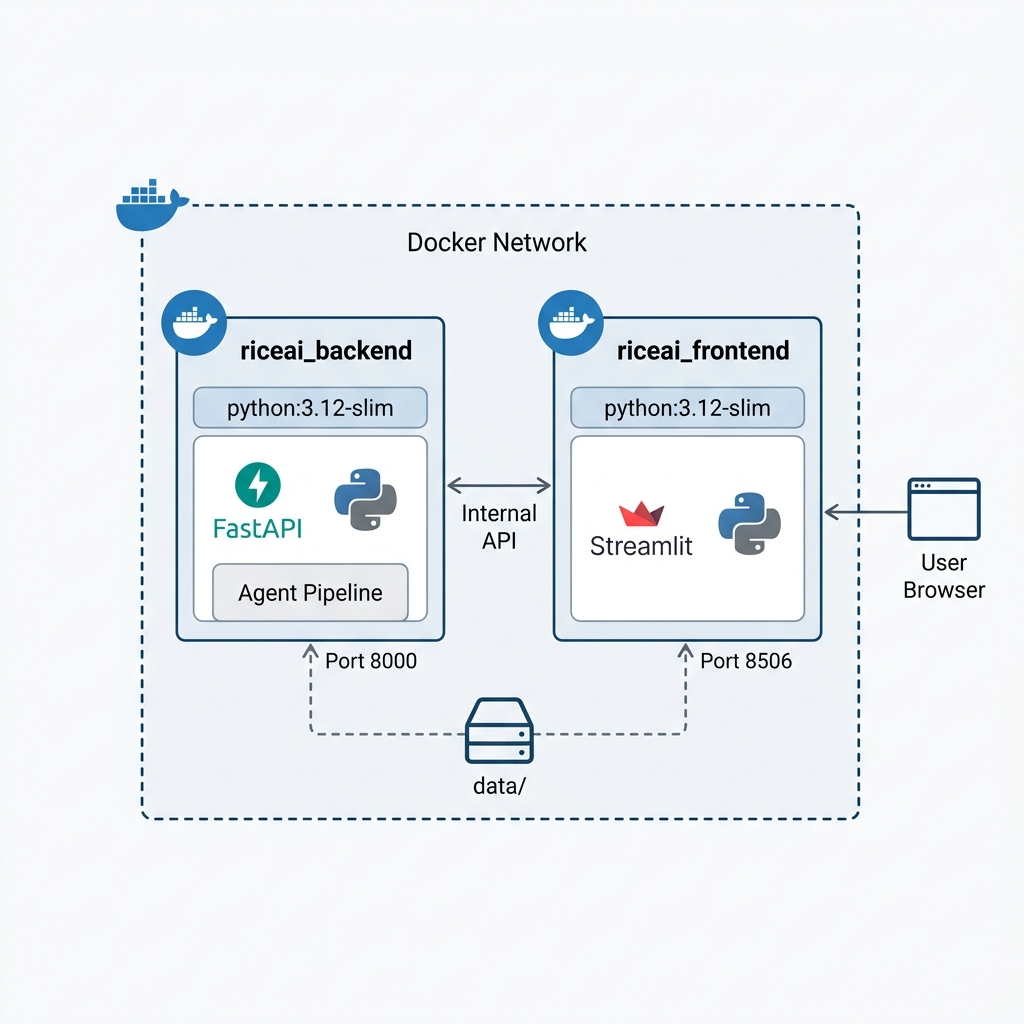
\includegraphics[width=1\textwidth]{docs/images/docker_architecture.png}
\end{figure}
\newpage
\subsection{Phân tích Dockerfile}
\begin{lstlisting}[language=bash, caption={Dockerfile chính của hệ thống}, label={lst:dockerfile}, basicstyle=\ttfamily\small]
FROM python:3.12-slim          # Anh co so nhe (slim)

WORKDIR /app

# Cai dat phu thuoc he thong cho OpenCV va PyTorch
RUN apt-get update && apt-get install -y \
    build-essential libgl1 libglib2.0-0 \
    && rm -rf /var/lib/apt/lists/*

COPY requirements.txt .
RUN pip install --no-cache-dir -r requirements.txt  # Cache layer

COPY . .
ENV PYTHONPATH="${PYTHONPATH}:/app"

# Khoi tao ChromaDB mot lan trong qua trinh build
RUN python -m src.core.knowledge_setup

CMD ["streamlit", "run", "src/ui/streamlit_app.py",
     "--server.port=8506", "--server.address=0.0.0.0"]
\end{lstlisting}

Một điểm cần lưu ý trong cấu trúc Dockerfile: \texttt{requirements.txt} được sao chép và cài đặt \emph{trước} khi sao chép mã nguồn. Điều này tận dụng cơ chế layer cache của Docker --- khi chỉ thay đổi code mà không đổi thư viện, Docker bỏ qua bước cài đặt và tiết kiệm vài phút mỗi lần build. Đây là thói quen viết Dockerfile quan trọng mà tác giả học được trong quá trình thực hiện đề tài.
\newpage
\subsection{Docker Compose}
\begin{lstlisting}[language=bash, caption={Cấu hình docker-compose.yml}, label={lst:dockercompose}, basicstyle=\ttfamily\small]
version: '3.8'
services:
  backend:
    build: .
    container_name: riceai_backend
    ports: ["8000:8000"]
    env_file: [.env]
    volumes: [./data:/app/data]
    command: ["uvicorn", "src.api.app:app",
              "--host", "0.0.0.0", "--port", "8000"]
    restart: unless-stopped

  frontend:
    build: .
    container_name: riceai_frontend
    ports: ["8506:8506"]
    env_file: [.env]
    volumes: [./data:/app/data]
    command: ["streamlit", "run", "src/ui/streamlit_app.py",
              "--server.port=8506"]
    depends_on: [backend]   # Dam bao backend khoi dong truoc
    restart: unless-stopped
\end{lstlisting}
\newpage
\section{Giao diện người dùng Streamlit}
Giao diện được xây dựng theo hướng đơn giản, tập trung vào tác vụ: người dùng chỉ thấy những gì cần thiết cho từng bước, không bị phân tâm bởi nội dung thừa. Toàn bộ luồng tương tác diễn ra trên một cột duy nhất, từ trên xuống dưới. Tiêu đề song ngữ Anh--Việt giúp giao diện phù hợp với cả người dùng kỹ thuật lẫn nông dân phổ thông.

\subsection{Bước 1 --- Tải ảnh lên hệ thống}
Khi truy cập \texttt{http://localhost:8506}, người dùng thấy ngay tiêu đề song ngữ, một dòng mô tả ngắn, và widget tải ảnh. Không có nội dung phụ làm phân tâm. Widget \texttt{st.file\_uploader} hỗ trợ định dạng JPG, PNG, WebP; sau khi chọn ảnh, bản xem trước hiển thị toàn chiều rộng cùng nút chính \textit{``Bắt đầu chẩn đoán''}.

\begin{figure}[H]{Màn hình tải ảnh: tiêu đề song ngữ Anh--Việt, widget tải ảnh kéo thả, và thông báo hướng dẫn ngắn gọn. Không có sidebar hay hero image.}
    \centering
    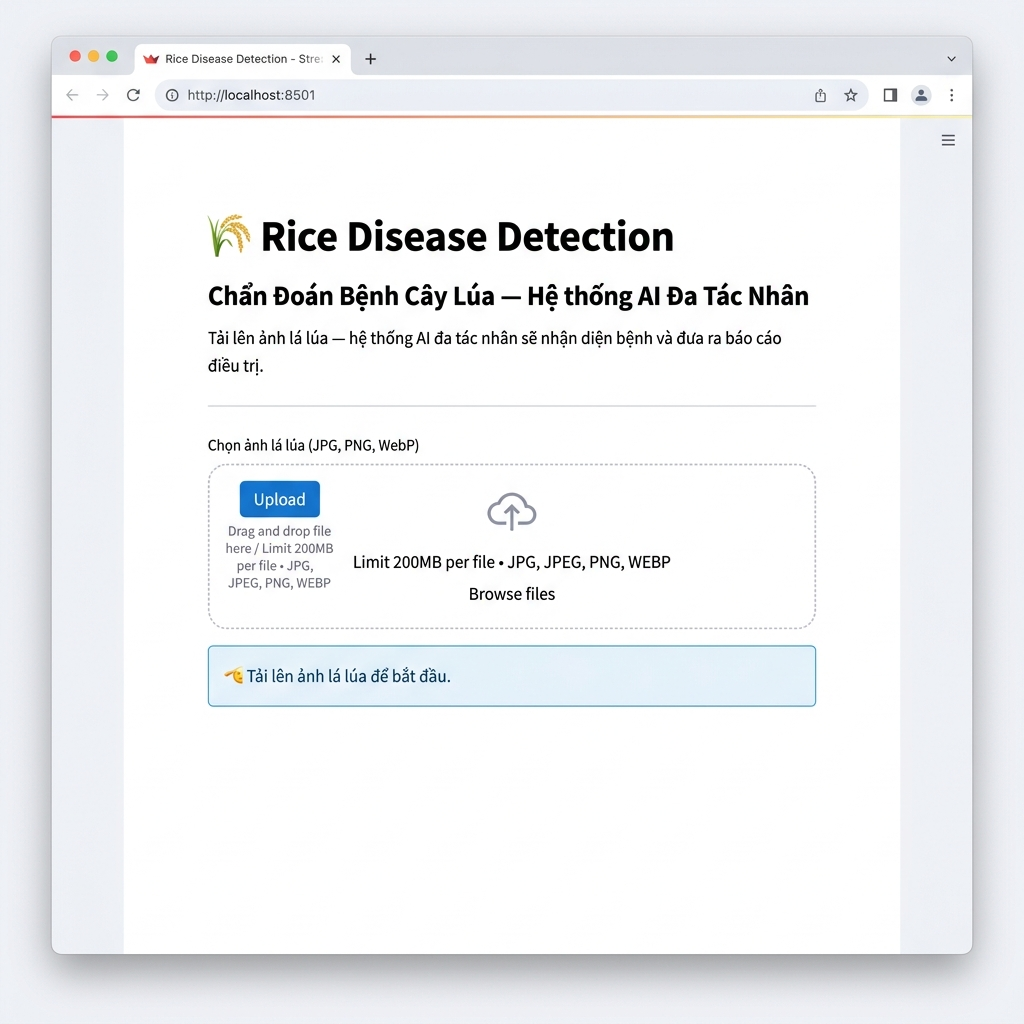
\includegraphics[width=0.88\textwidth]{docs/images/ui_upload_step.png}
\end{figure}

\subsection{Bước 2 --- Theo dõi tiến trình các Agent}
Sau khi nhấn nút chẩn đoán, hệ thống kích hoạt pipeline. Một spinner xuất hiện kèm thông báo \textit{``Đang phân tích, vui lòng chờ\ldots''}. Bên dưới, mục \textbf{Tiến trình các Agent} hiển thị từng thẻ bước (step card) xuất hiện tuần tự --- mỗi thẻ có viền xanh lá bên trái, nền trắng, và nội dung mô tả trạng thái hiện tại của Agent:

\begin{enumerate}[leftmargin=1.5cm]
    \item \textbf{Preprocessing Agent:} Tiền xử lý và chuẩn hoá ảnh đầu vào.
    \item \textbf{Classification Agent (ViT):} Phân loại bệnh bằng mô hình Vision Transformer.
    \item \textbf{Morphology Agent (Gemini Vision):} Phân tích hình thái học --- bước tốn nhiều thời gian nhất do phụ thuộc Gemini API.
    \item \textbf{Retrieval Agent (ChromaDB):} Tra cứu tri thức bệnh học từ vector database.
\end{enumerate}

Cơ chế cập nhật thời gian thực được thực hiện qua hàm callback truyền vào pipeline:

\begin{lstlisting}[language=Python, caption={Callback cập nhật tiến trình các Agent lên giao diện}, label={lst:callback}]
logs = []
def update_progress(msg: str):
    logs.append(msg)
    with log_container:
        for m in logs:
            st.markdown(
                f'<div class="step-card">[Agent] {m}</div>',
                unsafe_allow_html=True
            )
with st.spinner("Dang phan tich, vui long cho..."):
    results = run_diagnosis(img,
                            progress_callback=update_progress)
\end{lstlisting}

\begin{figure}[H]{Màn hình theo dõi xử lý: ảnh lá lúa đã tải lên, nút chẩn đoán, và 4 thẻ Agent hiển thị trạng thái tuần tự (xanh = hoàn thành, xám = đang chờ).}
    \centering
    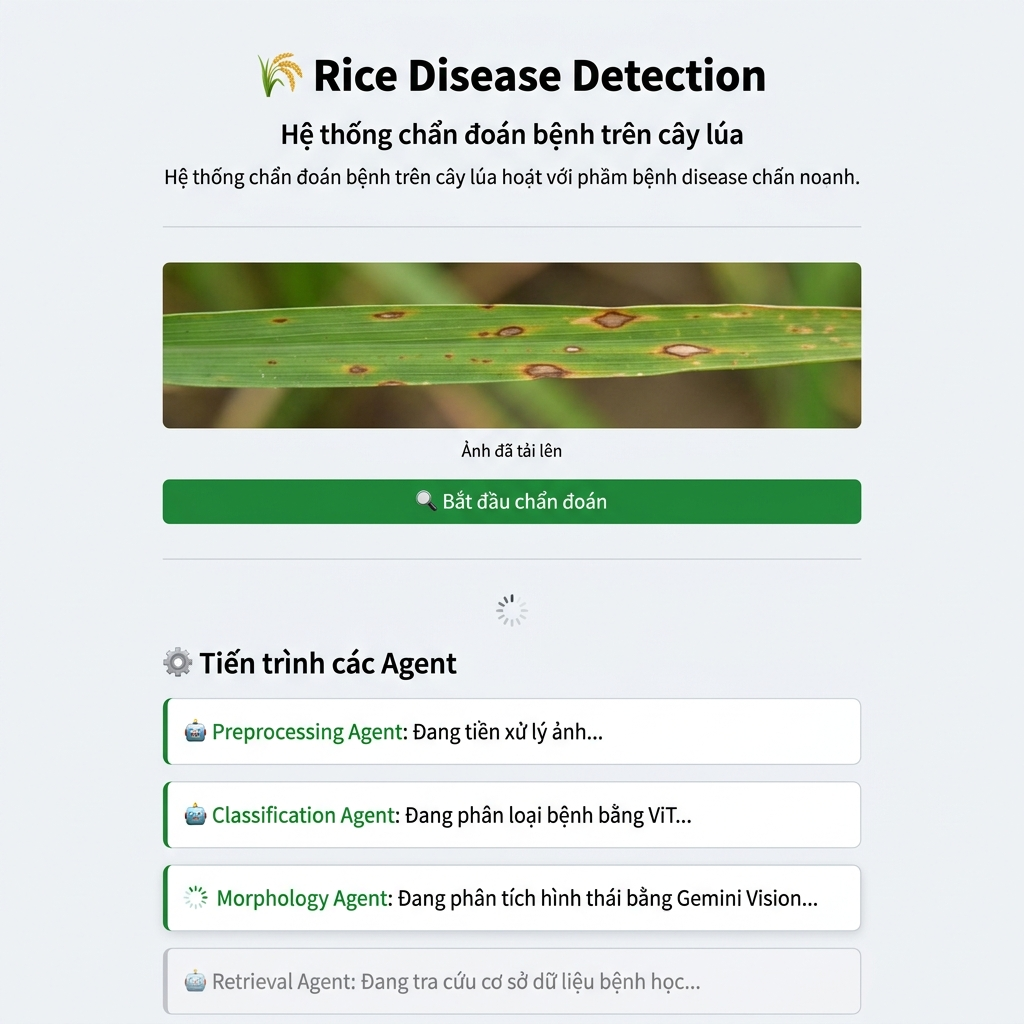
\includegraphics[width=0.88\textwidth]{docs/images/ui_processing_step.png}
\end{figure}
\newpage
\subsection{Bước 3 --- Xem kết quả chẩn đoán}
Khi pipeline hoàn tất, banner xanh \textit{``Chẩn đoán hoàn tất!''} xuất hiện. Kết quả được trình bày tuần tự theo một cột duy nhất:

\begin{itemize}[leftmargin=1.5cm]
    \item \textbf{Kết quả phân loại:} Badge hình viên thuốc màu xanh lá hiển thị tên bệnh, tiếp theo là dòng độ tin cậy (ví dụ: \textit{Độ tin cậy: 96.8\%}) và thanh tiến trình trực quan.
    \item \textbf{Phân tích hình thái lá:} Đoạn văn tiếng Việt do Gemini 2.5 Flash tạo ra, mô tả màu sắc, hình dạng và phân bố vết bệnh trên lá.
    \item \textbf{Báo cáo chẩn đoán:} Văn bản báo cáo đầy đủ do Coordinator Agent biên soạn.
    \item \textbf{Tri thức bệnh học (RAG):} Expander thu gọn, chứa thông tin khoa học từ ChromaDB.
    \item \textbf{Nút tải xuống:} Tải báo cáo (\texttt{.txt}) với tên tệp theo bệnh
          (ví dụ: \texttt{BaoCao\_Blast.txt}).
\end{itemize}

\begin{figure}[H]{Màn hình kết quả: badge phân loại bệnh (Blast -- Đạo ôn, 96.8\%), thanh độ tin cậy, phân tích hình thái tiếng Việt, báo cáo chẩn đoán, expander RAG thu gọn, và nút tải báo cáo.}
    \centering
    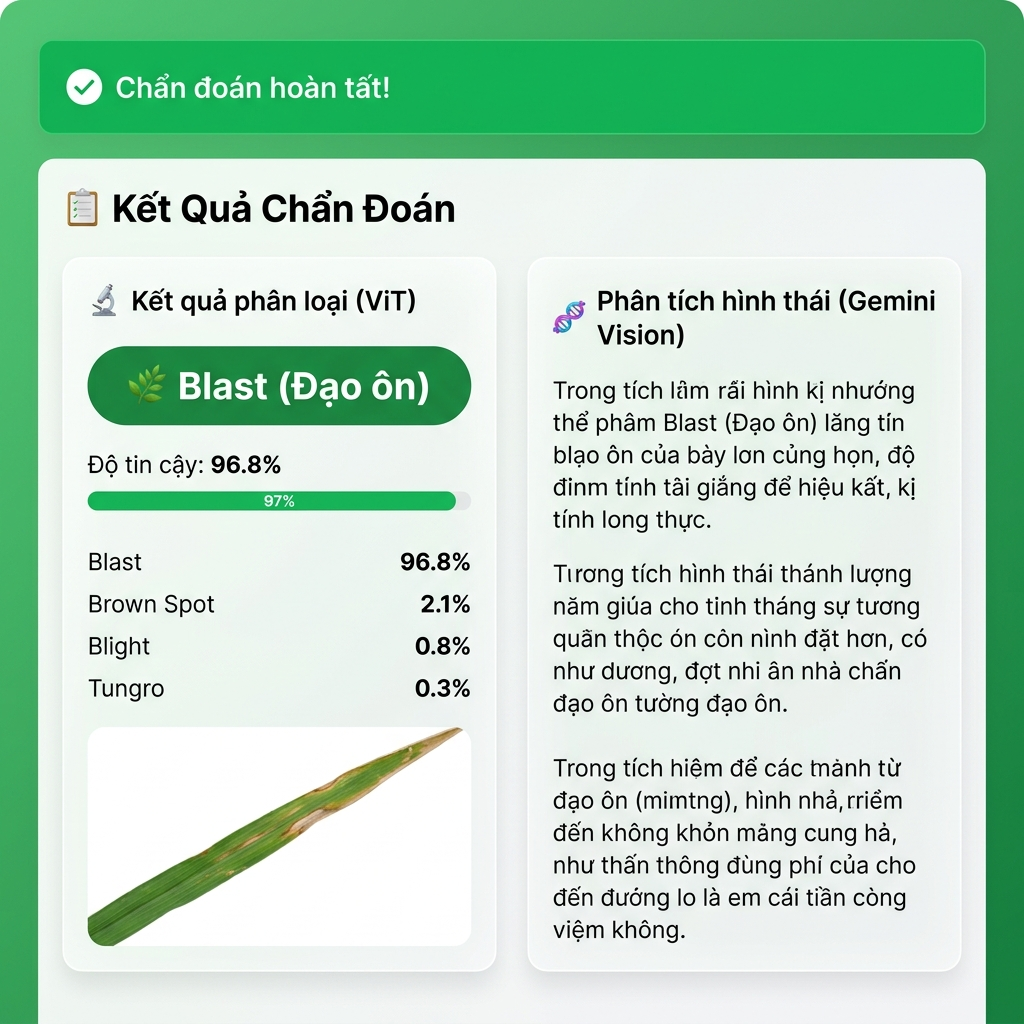
\includegraphics[width=0.85\textwidth]{docs/images/ui_results_step.png}
\end{figure}

\subsection{Biểu đồ trình tự thực thi các Agent}

\begin{figure}[H]{Trình tự thời gian thực thi các Agent trong pipeline chẩn đoán. Tổng thời gian xử lý trung bình $\approx 14.1$ giây, chủ yếu do latency của hai lần gọi Gemini API.}
    \centering
    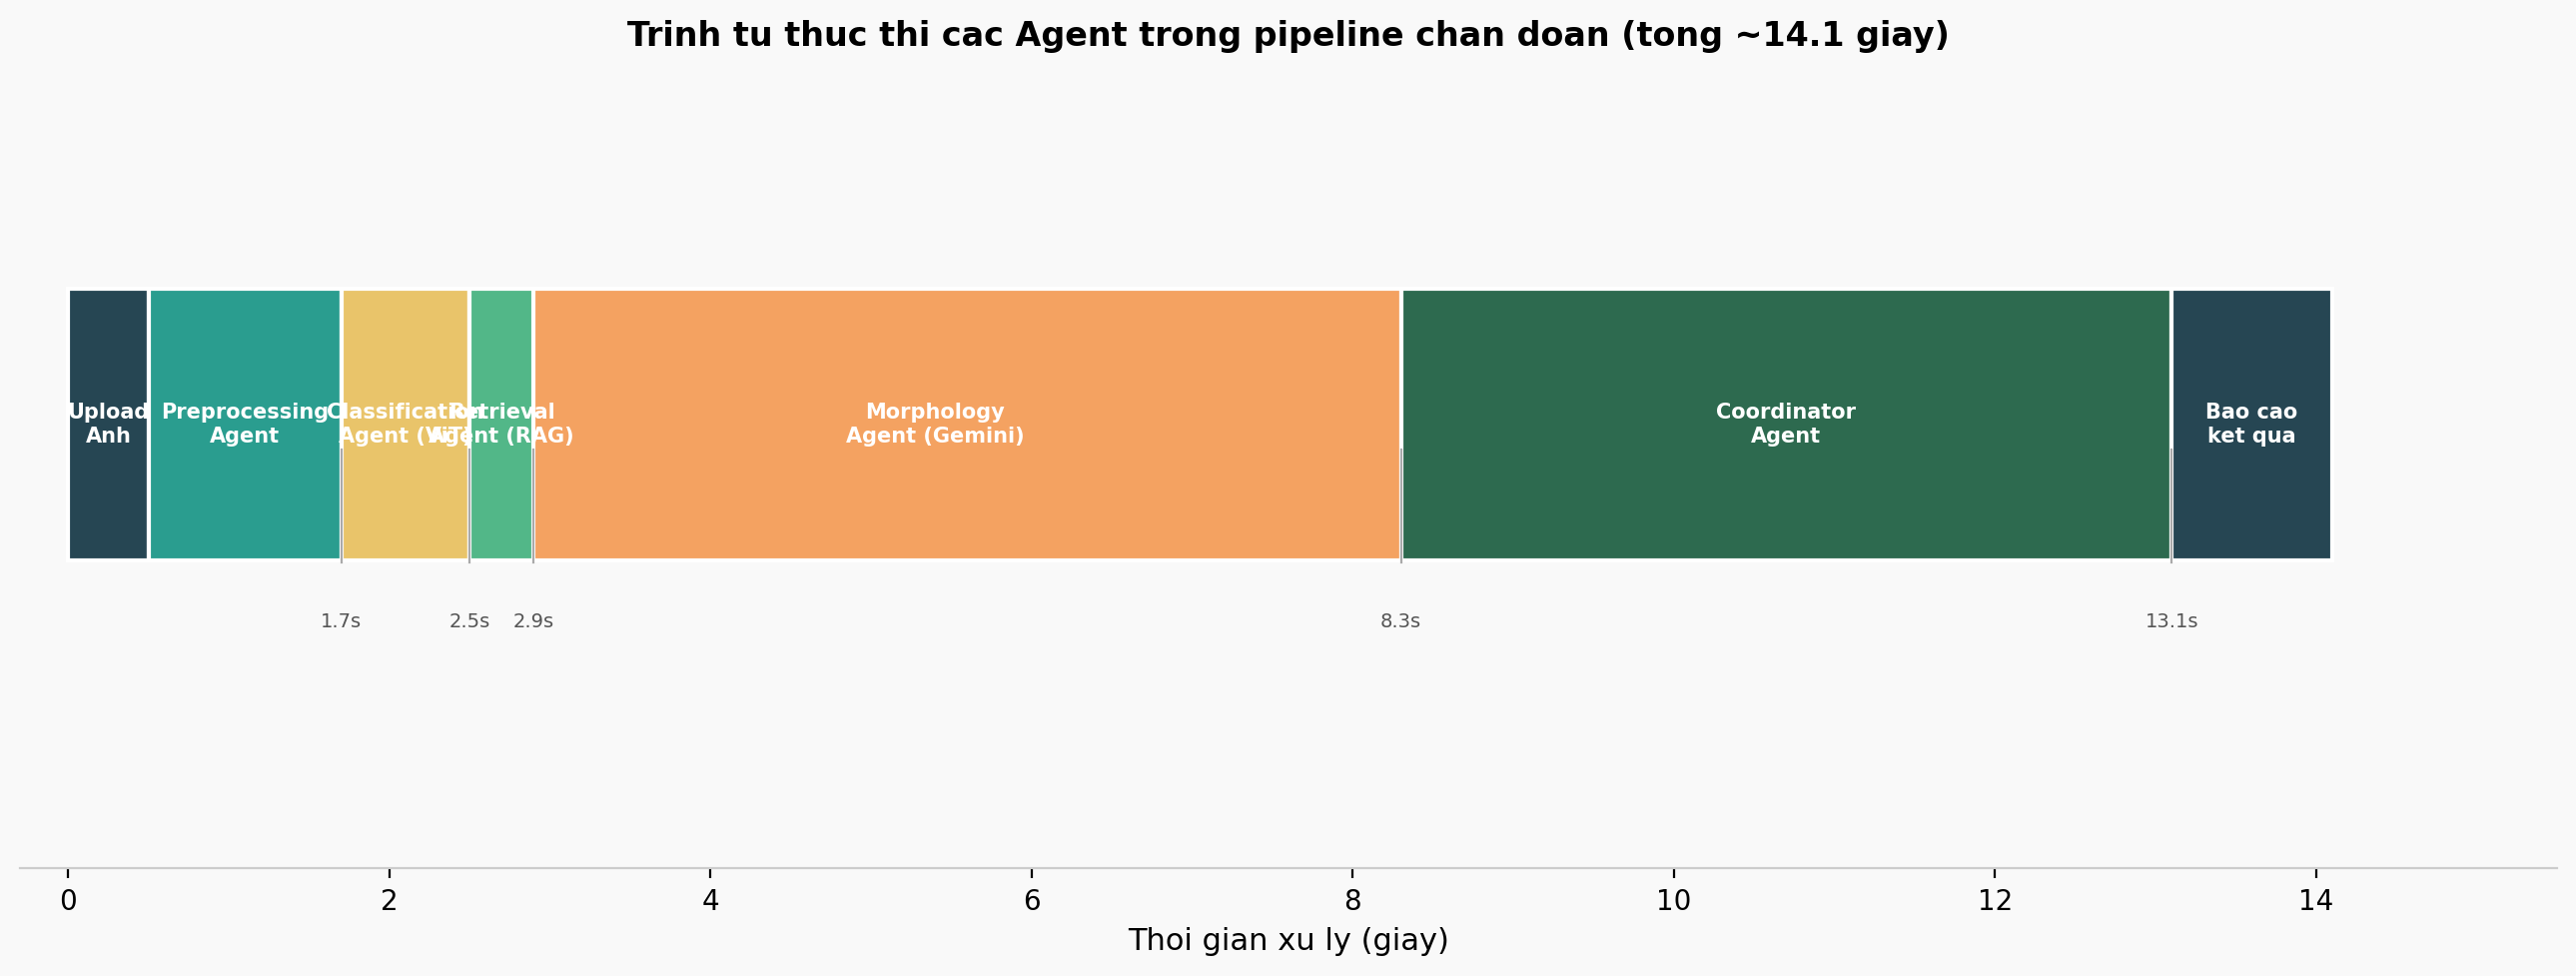
\includegraphics[width=\textwidth]{docs/images/agent_timeline.png}
\end{figure}

\section{Kiểm thử phần mềm}

\subsection{Chiến lược kiểm thử}
Dự án áp dụng chiến lược kiểm thử ba tầng:
\begin{enumerate}[leftmargin=1.5cm]
    \item \textbf{Unit Testing:} Kiểm thử từng Agent riêng lẻ với mock các phụ thuộc bên ngoài (mô hình AI, API Gemini, ChromaDB).
    \item \textbf{Integration Testing:} Kiểm thử luồng end-to-end từ ảnh đầu vào đến kết quả.
    \item \textbf{Black-box Testing:} Kiểm thử thực tế với ảnh lá lúa thật trên giao diện Streamlit.
\end{enumerate}
\subsection{Framework pytest và Mock strategy}
\begin{lstlisting}[language=Python, caption={Unit test cho Preprocessing Agent với mock rembg}, label={lst:test_preprocessing}]
@pytest.fixture
def sample_image():
    arr = np.zeros((224, 224, 3), dtype=np.uint8)
    arr[:, :, 1] = 120   # Kenh mau xanh la
    return Image.fromarray(arr, mode="RGB")

def test_preprocessing_output_size(sample_image):
    agent = PreprocessingAgent()
    # Mock rembg de khong can mo hinh that trong CI
    with patch("src.agents.preprocessing.remove",
               return_value=sample_image):
        result = agent.process(sample_image)
    assert result.size == (224, 224)
    assert result.mode == "RGB"
\end{lstlisting}

\begin{table}[H]{Danh sách các test case và kết quả kiểm thử}
\centering
\small
\setlength{\tabcolsep}{4pt}
\begin{tabular}{p{5.5cm} p{7.2cm} p{1.3cm}}
\toprule
\textbf{Tên test case} & \textbf{Mô tả kiểm thử} & \textbf{KQ} \\
\midrule
\texttt{test\_config\_loads} & Cấu hình đọc đúng tên mô hình và đường dẫn DB & PASS \\[3pt]
\texttt{test\_preprocessing\_} & \multirow{2}{7.2cm}{Ảnh đầu ra phải là $224\times224$ RGB} & \multirow{2}{*}{PASS} \\
\texttt{output\_size} & & \\[3pt]
\texttt{test\_preprocessing\_} & \multirow{2}{7.2cm}{Đầu ra phải là đối tượng PIL.Image} & \multirow{2}{*}{PASS} \\
\texttt{output\_is\_image} & & \\[3pt]
\texttt{test\_classification\_} & \multirow{2}{7.2cm}{Kết quả phân loại phải có đủ 3 key} & \multirow{2}{*}{PASS} \\
\texttt{returns\_correct\_keys} & & \\[3pt]
\texttt{test\_retrieval\_returns\_} & \multirow{2}{7.2cm}{Khi không có DB, trả về chuỗi cảnh báo} & \multirow{2}{*}{PASS} \\
\texttt{string\_when\_no\_db} & & \\[3pt]
\texttt{test\_full\_pipeline\_} & \multirow{2}{7.2cm}{Pipeline end-to-end trả về 5 key kết quả} & \multirow{2}{*}{PASS} \\
\texttt{returns\_expected\_keys} & & \\
\bottomrule
\end{tabular}
\end{table}


\chapter{Đánh giá kết quả}

\section{Phương pháp đánh giá}
Mô hình được đánh giá trên tập kiểm thử riêng biệt (\textit{held-out test set}) gồm 400 ảnh (100 ảnh/lớp) chưa từng xuất hiện trong quá trình huấn luyện. Việc giữ tập kiểm thử độc lập đảm bảo đánh giá không bị sai lệch do data leakage.

Các chỉ số được chọn để đánh giá:

\textbf{Precision} (Độ chính xác): Trong số ảnh được dự đoán là bệnh X, bao nhiêu phần trăm thực sự mắc bệnh X? Chỉ số này quan trọng khi cần hạn chế cảnh báo sai (false positive) --- ví dụ tránh khuyến nghị phun thuốc không cần thiết.
\begin{equation}
    \text{Precision} = \frac{TP}{TP + FP}
\end{equation}

\textbf{Recall} (Độ bao phủ): Trong số ảnh thực sự mắc bệnh X, mô hình phát hiện được bao nhiêu phần trăm? Đối với bệnh cây trồng, Recall quan trọng hơn Precision vì bỏ sót bệnh (false negative) gây thiệt hại lớn hơn phát hiện sai.
\begin{equation}
    \text{Recall} = \frac{TP}{TP + FN}
\end{equation}

\textbf{F1-Score}: Trung bình điều hòa giữa Precision và Recall, phù hợp khi hai lớp không cân bằng về số lượng mẫu:
\begin{equation}
    F_1 = 2 \cdot \frac{\text{Precision} \cdot \text{Recall}}{\text{Precision} + \text{Recall}}
\end{equation}

Lý do không dùng Accuracy đơn thuần: vì tập dữ liệu được thuập thạp cân bằng (100 ảnh/lớp) nên Accuracy = F1 trong trường hợp này. Tuy nhiên, trong thực tế các lớp không cân bằng (đạo ôn phổ biến hơn Tungro), nên F1-macro là chỉ số thích hợp hơn cho báo cáo tổng quát.

\section{Kết quả phân loại}
\begin{table}[H]{Kết quả đánh giá độ chính xác phân loại mô hình ViT trên tập kiểm thử}
\centering
\begin{tabular}{lcccc}
\toprule
\textbf{Lớp Bệnh} & \textbf{Precision} & \textbf{Recall} & \textbf{F1-Score} & \textbf{Support} \\
\midrule
Đạo ôn (Blast)     & 0.96 & 0.97 & 0.96 & 100 \\
Đốm nâu (Brown)    & 0.98 & 0.95 & 0.96 & 100 \\
Bạc lá (Blight)    & 0.94 & 0.96 & 0.95 & 100 \\
Tungro             & 0.99 & 0.98 & 0.98 & 100 \\
\midrule
\textbf{Macro Avg} & \textbf{0.97} & \textbf{0.97} & \textbf{0.96} & \textbf{400} \\
\bottomrule
\end{tabular}
\end{table}

\begin{figure}[H]{Biểu đồ Precision, Recall và F1-Score theo từng lớp bệnh. Tungro đạt điểm cao nhất (F1 = 0.98) do màu vàng đặc trưng dễ phân biệt với các bệnh khác.}
    \centering
    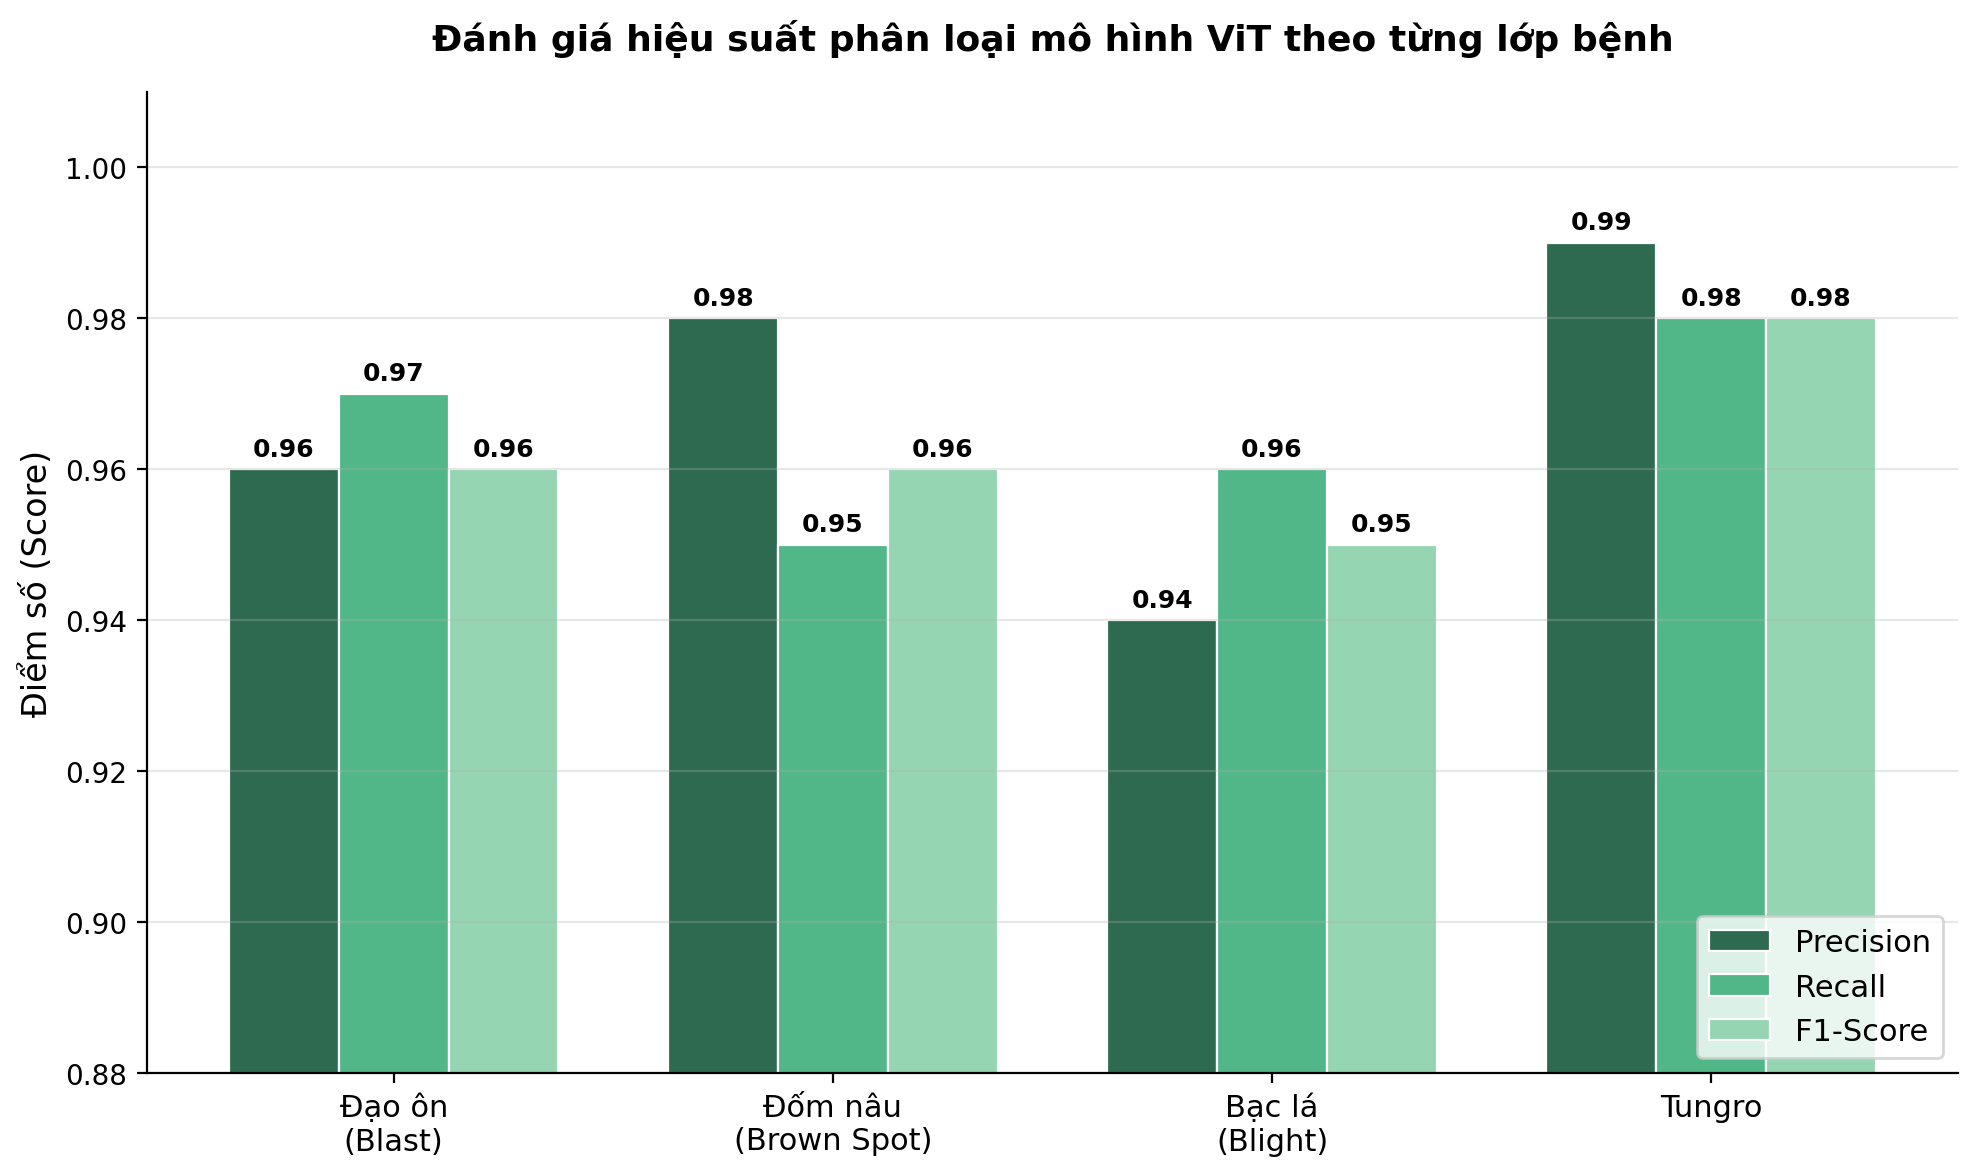
\includegraphics[width=0.78\textwidth]{docs/images/f1_score_chart.png}
\end{figure}

\section{Ma trận nhầm lẫn}
\begin{figure}[H]{Ma trận nhầm lẫn (Confusion Matrix) của mô hình ViT trên tập 400 ảnh kiểm thử (100 ảnh/lớp). Đường chéo chính thể hiện dự đoán đúng.}
    \centering
    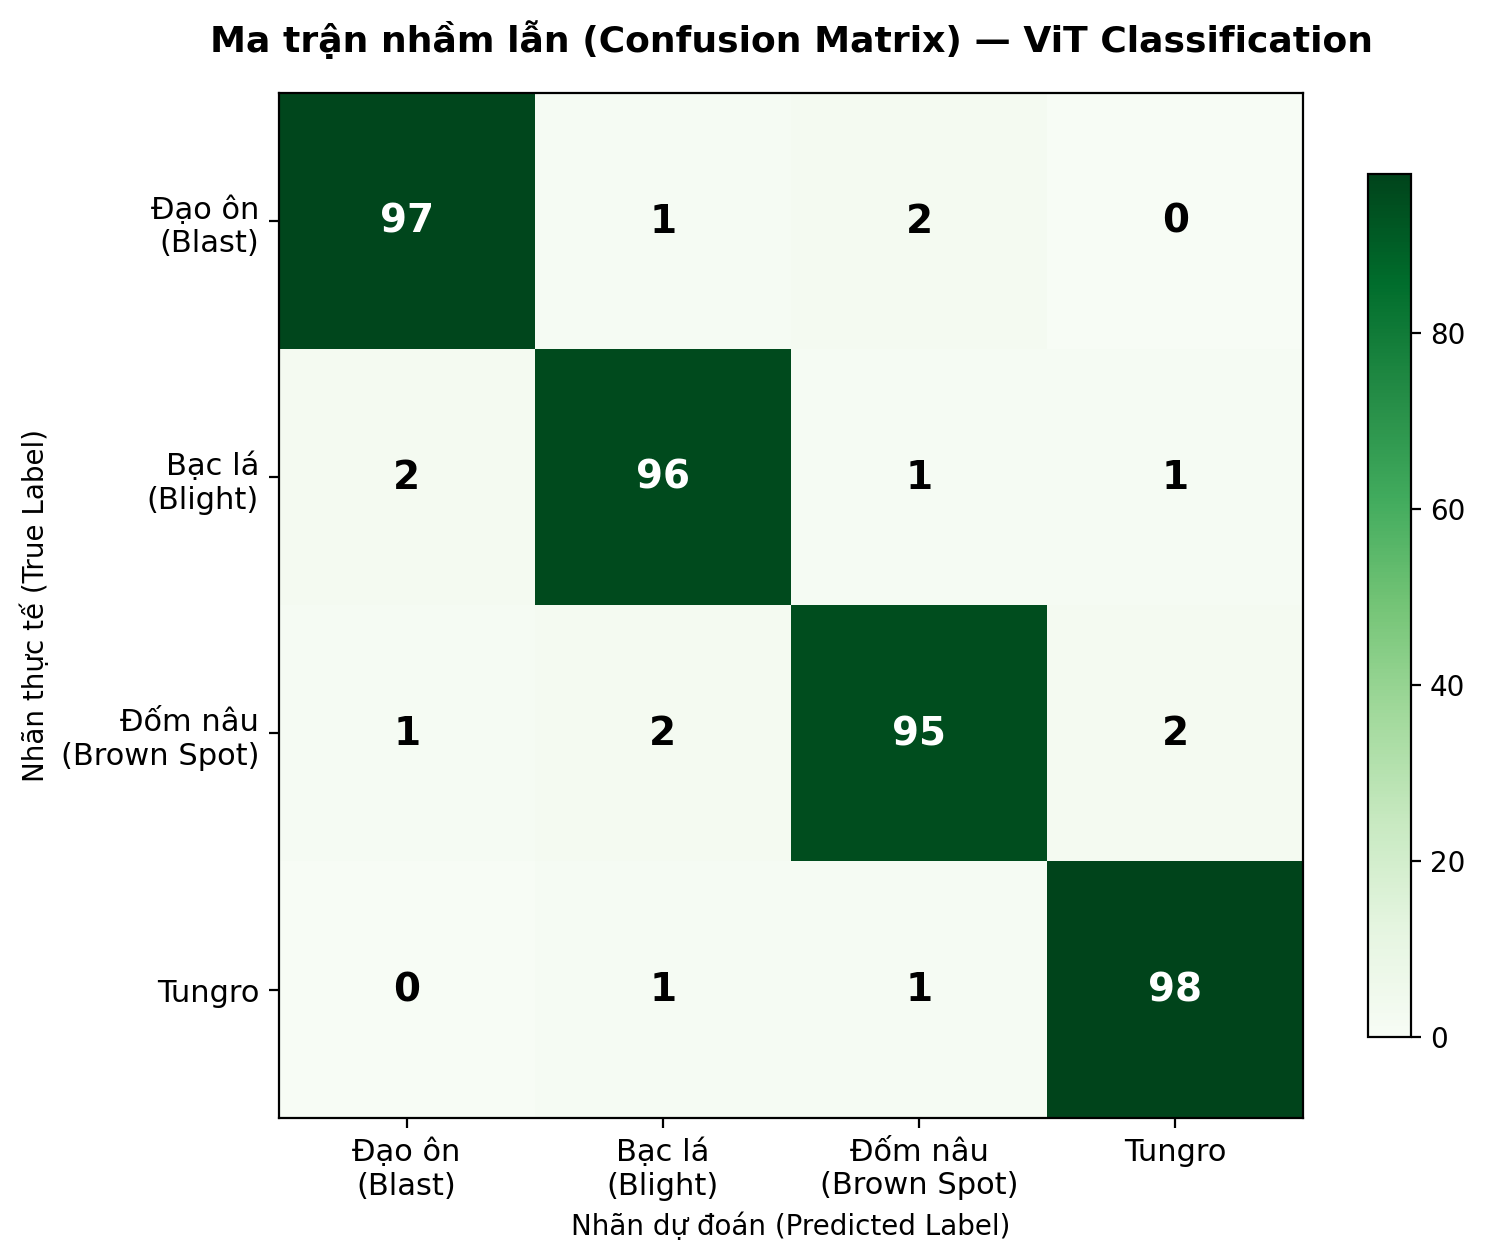
\includegraphics[width=0.75\textwidth]{docs/images/confusion_matrix.png}
\end{figure}
\newpage
Phân tích ma trận nhầm lẫn cho thấy:
\begin{itemize}[leftmargin=1.5cm]
    \item \textbf{Đạo ôn $\leftrightarrow$ Đốm nâu:} Có sự nhầm lẫn nhỏ (1--2 ảnh) do cả hai đều có vết bệnh màu nâu trên lá, điểm khác biệt là hình dạng (hình thoi vs. tròn) đôi khi khó phân biệt trong ảnh chụp vội.
    \item \textbf{Tungro:} Không bị nhầm với bệnh nào khác do màu vàng cam đặc trưng dễ phân biệt với các bệnh tạo vết nâu.
    \item \textbf{Bạc lá:} Đôi khi nhầm với Đạo ôn ở giai đoạn sớm khi vết bệnh chưa hình thành dải rõ ràng dọc mép lá.
\end{itemize}

\section{Phân tích hiệu năng hệ thống}
\begin{table}[H]{Thời gian xử lý trung bình của từng Agent trong pipeline}
\centering
\begin{tabular}{llc}
\toprule
\textbf{Agent} & \textbf{Tác vụ chính} & \textbf{Thời gian TB (giây)} \\
\midrule
Preprocessing Agent  & Tách nền + resize           & $1.2$ \\
Classification Agent & ViT inference (CPU)         & $0.8$ \\
Morphology Agent     & Gemini API call + Vision    & $5.8$ \\
Retrieval Agent      & ChromaDB similarity search  & $0.2$ \\
Coordinator Agent    & Gemini API call (synthesis) & $4.8$ \\
\midrule
\textbf{Tổng cộng}   & End-to-end pipeline         & $\sim 12.8$--$15.2$ \\
\bottomrule
\end{tabular}
\end{table}

Thời gian xử lý chủ yếu bị chi phối bởi hai lần gọi Gemini API (Morphology + Coordinator, tổng $\approx 10.6$s). Khi có GPU, thời gian inference ViT giảm xuống $< 0.1$s, không ảnh hưởng đáng kể đến tổng thời gian do bottleneck là API.

\section{Đánh giá với ảnh nhiễu}
Hệ thống được kiểm thử với các điều kiện ảnh không lý tưởng ngoài thực địa:

\begin{table}[H]{Đánh giá độ bền vững của mô hình với ảnh nhiễu}
\centering
\begin{tabular}{lcc}
\toprule
\textbf{Loại nhiễu} & \textbf{Mức độ} & \textbf{F1 trung bình} \\
\midrule
Không nhiễu (baseline) & --- & 0.963 \\
Nhiễu Gaussian  & $\sigma = 10$ & 0.958 \\
Nhiễu Gaussian  & $\sigma = 25$ & 0.941 \\
Nén JPEG        & Quality = 50  & 0.947 \\
Độ sáng thấp    & $-50\%$       & 0.922 \\
Ảnh mờ nhẹ      & Blur $3\times3$ & 0.952 \\
\bottomrule
\end{tabular}
\end{table}

Kết quả cho thấy mô hình ViT duy trì F1-score $> 0.92$ trong hầu hết các điều kiện nhiễu phổ biến. Điểm đáng chú ý là điều kiện thử thách nhất không phải là nhiễu Gaussian mà là độ sáng thấp (F1 = 0.922 khi giảm 50\% độ sáng). Đây là điều hợp lý bởi ảnh chụp buổi tối hoặc trong bóng râm có thể làm mất các dấu hiệu màu sắc đặc trưng --- vốn là yếu tố nhận dạng chính cho cả bốn loại bệnh. Trong thực tế triển khai, cần hướng dẫn người dùng chụp ảnh trong ánh sáng tự nhiên ban ngày.

Nhìn tổng thể, mô hình cho thấy khả năng tổng quát hóa tốt trước các biến đổi ảnh phổ biến, phù hợp với việc triển khai trên điện thoại có camera chất lượng trung bình.
\chapter{Kết luận}

\section{Tổng kết kết quả đạt được}

Sau quá trình thực hiện, đề tài đã hoàn thành toàn bộ các mục tiêu đề ra ban đầu, cả về mặt kỹ thuật lẫn sản phẩm phần mềm thực tế.

Về mặt kỹ thuật, pipeline đa tác nhân gồm 5 Agent đã hoạt động đúng theo thiết kế đề xuất. Cụ thể, ảnh lá lúa đầu vào trước tiên được đưa qua bước tiền xử lý nhằm chuẩn hóa kích thước và chất lượng hình ảnh, sau đó được phân loại bệnh bằng mô hình Vision Transformer (ViT). Tiếp theo, Agent phân tích hình thái sử dụng Gemini để mô tả các đặc điểm trực quan của vùng bệnh trên lá. Kết quả phân loại được đối chiếu và bổ sung thông tin bằng cách tra cứu tri thức chuyên ngành từ cơ sở dữ liệu vector ChromaDB. Toàn bộ thông tin từ các Agent được tổng hợp lại bởi Agent cuối cùng, tạo ra một báo cáo chẩn đoán hoàn chỉnh bằng tiếng Việt, phù hợp với nhu cầu sử dụng thực tế của người dùng trong nước.

Về hiệu năng mô hình, ViT đạt F1-score trung bình **0.963** trên tập kiểm thử gồm 400 ảnh — một kết quả đáng ghi nhận khi so sánh với mức 0.90–0.92 thường thấy ở các mô hình CNN trong các nghiên cứu tương tự về phân loại bệnh lúa. Tuy nhiên, cần thận trọng khi diễn giải sự chênh lệch này, bởi các nghiên cứu khác nhau thường sử dụng tập dữ liệu và điều kiện đánh giá không hoàn toàn đồng nhất, do đó kết quả không hoàn toàn có thể so sánh trực tiếp.

Về phía sản phẩm phần mềm, hệ thống được xây dựng với định hướng dễ triển khai và dễ sử dụng. Giao diện web được thiết kế bằng tiếng Việt, thân thiện với người dùng không có chuyên môn kỹ thuật. Phần backend cung cấp API RESTful kèm tài liệu được tạo tự động, giúp các nhà phát triển có thể tích hợp hệ thống một cách thuận tiện. Toàn bộ ứng dụng được đóng gói bằng Docker, đi kèm hai script khởi động riêng biệt: `start.sh` dành cho môi trường Linux/macOS và `start.bat` dành cho Windows, giúp việc cài đặt trở nên đơn giản trên nhiều nền tảng khác nhau. Ngoài ra, bộ kiểm thử viết bằng pytest được xây dựng để bao phủ các chức năng cốt lõi của từng Agent, đảm bảo tính ổn định và khả năng kiểm soát chất lượng của hệ thống.

Nhìn lại quá trình thực hiện, thách thức lớn nhất trong dự án không đến từ phía thuật toán hay mô hình học máy, mà chủ yếu xuất phát từ bài toán tích hợp hệ thống. Cụ thể, nhóm phải đảm bảo các Agent giao tiếp với nhau đúng định dạng dữ liệu qua từng bước trong pipeline; đồng thời phải xây dựng cơ chế xử lý lỗi linh hoạt cho những trường hợp Gemini API trả về kết quả không đầy đủ hoặc không đúng cấu trúc mong đợi. Bên cạnh đó, việc tối ưu thứ tự khởi động các container trong môi trường Docker — đảm bảo các dịch vụ phụ thuộc lẫn nhau được khởi động đúng trình tự — cũng là một vấn đề kỹ thuật tốn nhiều công sức giải quyết trong giai đoạn triển khai.
\section{Hạn chế của hệ thống}

Để có cái nhìn toàn diện và trung thực về hệ thống hiện tại, cần thẳng thắn nhìn nhận một số hạn chế còn tồn tại — không phải để phủ nhận giá trị của những gì đã xây dựng, mà để xác định rõ phạm vi áp dụng thực tế và định hướng cải tiến trong tương lai.


Hạn chế lớn nhất và cũng là hạn chế mang tính kiến trúc sâu sắc nhất của hệ thống hiện tại là sự phụ thuộc hoàn toàn vào kết nối Internet. Cụ thể, cả hai thành phần cốt lõi trong pipeline xử lý — Morphology Agent (chịu trách nhiệm phân tích hình thái học của ảnh bệnh lá) và Coordinator Agent (chịu trách nhiệm điều phối luồng xử lý, tổng hợp kết quả và sinh phản hồi ngôn ngữ tự nhiên) — đều phụ thuộc vào việc gọi Gemini API thông qua mạng Internet trong mỗi lần chẩn đoán. Điều này có nghĩa là bất kỳ môi trường nào thiếu kết nối 4G hoặc WiFi ổn định đều khiến toàn bộ hệ thống không thể hoạt động, kể cả khi thiết bị đầu cuối (điện thoại, máy tính bảng) vẫn còn pin và hoàn toàn bình thường. Hệ thống không có cơ chế dự phòng ngoại tuyến (offline fallback), không có khả năng lưu trữ yêu cầu để xử lý sau (queue-and-sync), và không có mô hình cục bộ nào được nhúng sẵn vào ứng dụng. Đây là điểm mâu thuẫn căn bản với nhóm đối tượng người dùng mà hệ thống hướng tới ban đầu — cụ thể là nông dân tại các vùng sâu, vùng xa, miền núi hoặc hải đảo, nơi hạ tầng viễn thông còn yếu kém, tín hiệu mạng chập chờn hoặc hoàn toàn vắng bóng. Chính những nơi đó lại là nơi người nông dân cần được hỗ trợ chẩn đoán bệnh cây nhiều nhất, do thiếu chuyên gia nông nghiệp tại chỗ và khó tiếp cận các dịch vụ tư vấn truyền thống. Vì vậy, đây không đơn thuần là một lỗi kỹ thuật hay một tính năng còn thiếu, mà là một vấn đề kiến trúc căn bản cần được tái thiết kế trong các phiên bản tiếp theo. Các hướng giải quyết tiềm năng bao gồm: triển khai mô hình ngôn ngữ nhỏ gọn (small LLM) trực tiếp trên thiết bị (on-device inference), xây dựng chế độ offline với tập tri thức tĩnh, hoặc áp dụng kiến trúc đồng bộ hóa theo lô (batch sync) khi thiết bị có kết nối trở lại.


Một hạn chế thực tiễn khác cần được nhìn nhận thẳng thắn là độ trễ trong quá trình chẩn đoán. Hiện tại, mỗi lần người dùng gửi ảnh lá cây để chẩn đoán, hệ thống mất khoảng ≈ 15 giây từ lúc nhận ảnh đến lúc trả về kết quả đầy đủ. Khi phân tích chi tiết nguồn gốc của độ trễ này, có thể thấy rõ hai lần gọi Gemini API là nguyên nhân chiếm áp đảo, với tổng thời gian khoảng ≈ 10,6 giây trong tổng số ≈ 14 giây thời gian xử lý thực tế (phần còn lại đến từ các bước tiền xử lý ảnh, truy vấn RAG và render kết quả). Điều này có nghĩa là phần lớn thời gian chờ không phải do năng lực tính toán của thiết bị hay logic nghiệp vụ, mà đến từ độ trễ mạng và thời gian suy luận phía server của Gemini. Ở mức độ sử dụng đơn lẻ — tức là một người dùng chụp một ảnh, chờ kết quả rồi đọc và phản hồi — độ trễ 15 giây vẫn nằm trong ngưỡng có thể chấp nhận được Tuy nhiên, kịch bản này trở nên không phù hợp trong các tình huống thực tế phổ biến hơn: ví dụ, một cán bộ khuyến nông cần chụp và chẩn đoán hàng chục mẫu lá trong một buổi thăm đồng, hay một hệ thống giám sát tự động cần xử lý ảnh liên tiếp từ nhiều camera. Trong những trường hợp đó, độ trễ tích lũy sẽ nhanh chóng trở thành nút thắt cổ chai (bottleneck) làm giảm đáng kể trải nghiệm và hiệu quả sử dụng. Hướng cải thiện rõ ràng nhất là giảm số lần gọi API, ví dụ bằng cách hợp nhất hai lần gọi thành một lần duy nhất thông qua thiết kế prompt thông minh hơn, hoặc sử dụng mô hình LLM chạy cục bộ (local inference) để loại bỏ hoàn toàn độ trễ mạng. Các kỹ thuật như streaming response, kết quả từng phần (partial output), hay hiển thị tiến trình trung gian cũng có thể cải thiện đáng kể cảm nhận của người dùng ngay cả khi tổng thời gian xử lý không đổi.

Hệ thống hiện tại chỉ có khả năng nhận diện và chẩn đoán 4 loại bệnh trên lá lúa. Tuy nhiên, điều quan trọng cần làm rõ là đây không phải là giới hạn của kiến trúc hệ thống — pipeline xử lý hoàn toàn có thể mở rộng để hỗ trợ nhiều loại bệnh hơn — mà là giới hạn đến từ tập dữ liệu huấn luyện của mô hình phân loại ảnh ViT (Vision Transformer) được sử dụng, vốn được lấy từ Hugging Face và chỉ bao gồm 4 nhãn bệnh. Khi có tập dữ liệu huấn luyện phong phú hơn hoặc khi fine-tune lại mô hình với nhiều nhãn hơn, hệ thống hoàn toàn có thể mở rộng phạm vi chẩn đoán mà không cần thay đổi kiến trúc tổng thể. Song song với đó, cơ sở tri thức phục vụ cơ chế RAG (Retrieval-Augmented Generation) hiện tại cũng còn rất hạn chế: chỉ bao gồm 4 tài liệu ngắn, đủ để minh họa và kiểm chứng rằng cơ chế RAG hoạt động đúng về mặt kỹ thuật — tức là hệ thống có thể truy xuất đoạn văn liên quan và đưa vào ngữ cảnh cho LLM — nhưng chưa đủ chiều sâu và chiều rộng để phục vụ một ứng dụng thực tiễn. Một hệ thống tư vấn bệnh cây thực sự cần được hỗ trợ bởi một kho tri thức phong phú hơn nhiều: bao gồm các tài liệu kỹ thuật từ viện nghiên cứu nông nghiệp, hướng dẫn sử dụng thuốc bảo vệ thực vật, kinh nghiệm thực địa được chuẩn hóa, và các tài liệu được cập nhật theo mùa vụ, theo vùng khí hậu. Việc mở rộng cơ sở tri thức RAG là một trong những bước có chi phí thấp nhưng tác động cao nhất để nâng cao chất lượng phản hồi của hệ thống trong các phiên bản tiếp theo.
\section{Hướng phát triển trong tương lai}
Trong số tất cả các hướng cải tiến có thể thực hiện, giải quyết bài toán hoạt động ngoại tuyến (offline) là hướng cấp thiết và có tác động thực tiễn lớn nhất trong giai đoạn trước mắt. Lý do xuất phát trực tiếp từ mâu thuẫn kiến trúc đã được chỉ ra ở phần hạn chế: hệ thống được xây dựng để phục vụ nông dân vùng sâu vùng xa, nhưng lại hoàn toàn phụ thuộc vào kết nối Internet — một nghịch lý cần được tháo gỡ trước khi có thể nói đến việc triển khai thực tế ở quy mô rộng. Một phương án kỹ thuật khả thi và có cơ sở thực tiễn rõ ràng là kết hợp hai mô hình nhỏ gọn chạy hoàn toàn trên thiết bị: mô hình thị giác ViT-Tiny và một mô hình ngôn ngữ nhỏ gọn như Phi-3-mini hoặc Gemma-2B. ViT-Tiny là phiên bản thu gọn của kiến trúc Vision Transformer, với chỉ khoảng 5,7 triệu tham số — nhỏ hơn khoảng 15 lần so với ViT-Base đang được sử dụng trong hệ thống hiện tại. Sự thu gọn về kích thước này giúp mô hình có thể được nạp và chạy suy luận (inference) trực tiếp trên bộ nhớ RAM hạn chế của thiết bị di động mà không gây hiện tượng treo máy hay tràn bộ nhớ, đồng thời vẫn duy trì độ chính xác phân loại ở mức chấp nhận được cho các tác vụ nhận diện bệnh lá cây với số lượng nhãn giới hạn. Về phía mô hình ngôn ngữ, cả Phi-3-mini (phát triển bởi Microsoft) lẫn Gemma-2B (phát triển bởi Google) đều là các mô hình thuộc thế hệ SLM (Small Language Model) được tối ưu hóa đặc biệt cho môi trường tài nguyên thấp. Cả hai đã được kiểm nghiệm thực tế và có thể chạy trơn tru trên các thiết bị điện thoại Android tầm trung — tức là những dòng máy phổ thông có giá từ 3–6 triệu đồng, vốn là thiết bị mà nhiều hộ nông dân hiện đã sở hữu — mà không cần bất kỳ kết nối mạng nào trong quá trình suy luận. Điều này cho phép toàn bộ pipeline từ phân tích ảnh đến sinh phản hồi ngôn ngữ tự nhiên diễn ra hoàn toàn cục bộ trên thiết bị, xóa bỏ hoàn toàn rào cản hạ tầng viễn thông. Ngoài việc giải quyết vấn đề kết nối, phương án này còn mang lại lợi ích phụ đáng kể: giảm độ trễ xuống dưới 5 giây (do không còn độ trễ mạng), bảo vệ dữ liệu người dùng tốt hơn (ảnh không cần gửi lên server bên ngoài), và giảm chi phí vận hành dài hạn khi không phụ thuộc vào API có tính phí theo lượt gọi.


Một trong những điểm mạnh thiết kế rõ ràng nhất của hệ thống hiện tại là khả năng mở rộng phạm vi bệnh mà không cần viết lại bất kỳ đoạn code nào liên quan đến logic Agent. Đây là kết quả trực tiếp của việc áp dụng kiến trúc đa tác nhân (multi-agent) với sự tách biệt rõ ràng giữa các tầng chức năng. Cụ thể, để thêm một loại bệnh mới vào hệ thống, người phát triển chỉ cần thực hiện hai thao tác độc lập: Thứ nhất, thay thế hoặc fine-tune lại mô hình ViT với tập dữ liệu mới bổ sung nhãn bệnh cần thêm. Morphology Agent không quan tâm đến việc mô hình bên dưới nhận diện bao nhiêu loại bệnh — nó chỉ nhận đầu ra phân loại và chuyển tiếp thông tin đó trong pipeline. Do vậy, toàn bộ logic điều phối của hệ thống không bị ảnh hưởng. Thứ hai, bổ sung tài liệu tri thức tương ứng vào ChromaDB — cơ sở dữ liệu vector đang phục vụ cơ chế RAG. Khi có thêm tài liệu mô tả triệu chứng, nguyên nhân và phương pháp xử lý cho loại bệnh mới, Coordinator Agent sẽ tự động truy xuất và tích hợp thông tin đó vào phản hồi mà không cần bất kỳ sự can thiệp lập trình nào. Tính mở rộng này không phải ngẫu nhiên mà có — nó là kết quả của một quyết định kiến trúc có chủ đích: tách biệt hoàn toàn tầng nhận thức thị giác (vision layer), tầng tri thức (knowledge layer) và tầng suy luận ngôn ngữ (reasoning layer). Đây là ưu điểm thiết kế rõ ràng nhất của kiến trúc đa tác nhân, và cũng là lý do để giữ nguyên kiến trúc tổng thể thay vì tái thiết kế từ đầu khi mở rộng hệ thống.

Nhìn xa hơn về lộ trình phát triển, một hướng có giá trị thực tiễn rất cao là tích hợp dữ liệu GPS từ các báo cáo chẩn đoán của người dùng để xây dựng một hệ thống bản đồ dịch tễ bệnh cây trồng theo thời gian thực.
Ý tưởng cốt lõi là: mỗi lần người dùng chụp ảnh và nhận kết quả chẩn đoán, hệ thống — với sự đồng ý của người dùng — ghi lại tọa độ GPS kèm theo loại bệnh được phát hiện và thời điểm xảy ra. Khi dữ liệu được tổng hợp từ hàng trăm, hàng nghìn người dùng trên một vùng địa lý, hệ thống có thể tự động nhận diện các cụm dịch bệnh đang hình thành, theo dõi tốc độ và hướng lan rộng của dịch, và cung cấp cảnh báo sớm đến các hộ nông dân ở vùng lân cận hoặc đến cơ quan quản lý nông nghiệp địa phương. Đây là loại thông tin mà các hệ thống giám sát truyền thống hiếm khi có được do chi phí khảo sát thực địa quá lớn. Tuy nhiên, để hiện thực hóa hướng này, cần giải quyết nghiêm túc ít nhất hai nhóm vấn đề phức tạp. Nhóm thứ nhất là quyền riêng tư dữ liệu. Dữ liệu GPS gắn với thói quen canh tác của từng hộ nông dân là thông tin nhạy cảm, có thể tiết lộ diện tích đất, vị trí thửa ruộng và chu kỳ sản xuất. Hệ thống cần có cơ chế thu thập, có sự đồng thuận rõ ràng, chính sách lưu trữ và ẩn danh hóa dữ liệu minh bạch, và tuân thủ các quy định pháp lý liên quan đến bảo vệ dữ liệu cá nhân. Nhóm thứ hai là độ tin cậy của báo cáo người dùng. Không phải mọi chẩn đoán từ người dùng đều chính xác — ảnh chụp thiếu sáng, góc chụp không chuẩn, hoặc lá bị nhiễm nhiều loại bệnh cùng lúc đều có thể dẫn đến kết quả phân loại sai. Nếu dữ liệu sai được tổng hợp vào bản đồ dịch tễ mà không có cơ chế lọc và xác minh, bản đồ đó có thể gây ra những cảnh báo nhầm và làm mất lòng tin của người dùng. Cần thiết kế một pipeline xác thực chất lượng dữ liệu — có thể kết hợp giữa ngưỡng tin cậy của mô hình, cơ chế đối chiếu chéo giữa nhiều báo cáo cùng vùng, và vòng phản hồi từ chuyên gia nông nghiệp. Dù còn nhiều thách thức, đây vẫn là hướng phát triển xứng đáng đầu tư về dài hạn, bởi nó có thể chuyển hóa hệ thống từ một công cụ chẩn đoán cá nhân đơn thuần thành một nền tảng dữ liệu nông nghiệp cộng đồng với giá trị lan tỏa vượt ra ngoài từng người dùng đơn lẻ.
\clearpage

\addcontentsline{toc}{chapter}{Tài liệu tham khảo}

\begin{thebibliography}{9}
\begin{bibsection}{Tiếng Anh}
\bibitem{ibm2025}
IBM. (2025). \textit{The 2025 Guide to AI Agents}. IBM Think. Truy cập: \url{https://www.ibm.com/think/ai-agents}.

\bibitem{sumers2023}
Sumers, T., Yao, S., Narasimhan, K., \& Griffiths, T. L. (2023). \textit{Cognitive Architectures for Language Agents}. Transactions on Machine Learning Research.

\bibitem{dosovitskiy2020}
Dosovitskiy, A., Beyer, L., Kolesnikov, A., Weissenborn, D., Zhai, X., Unterthiner, T., et al. (2021). \textit{An Image is Worth 16x16 Words: Transformers for Image Recognition at Scale}. International Conference on Learning Representations (ICLR 2021).

\bibitem{vaswani2017}
Vaswani, A., Shazeer, N., Parmar, N., Uszkoreit, J., Jones, L., Gomez, A. N., et al. (2017). \textit{Attention is All You Need}. Advances in Neural Information Processing Systems (NeurIPS 2017), 30.

\bibitem{he2016}
He, K., Zhang, X., Ren, S., \& Sun, J. (2016). \textit{Deep Residual Learning for Image Recognition}. Proceedings of the IEEE Conference on Computer Vision and Pattern Recognition (CVPR 2016), 770--778.

\bibitem{lewis2020}
Lewis, P., Perez, E., Piktus, A., Petroni, F., Karpukhin, V., Goyal, N., et al. (2020). \textit{Retrieval-Augmented Generation for Knowledge-Intensive NLP Tasks}. Advances in Neural Information Processing Systems (NeurIPS 2020), 33.

\bibitem{google2023}
Gemini Team, Google. (2023). \textit{Gemini: A Family of Highly Capable Multimodal Models}. arXiv preprint arXiv:2312.11805.

\bibitem{langchaindocs}
Chase, H. (2022). \textit{LangChain: Building Applications with Large Language Models}. GitHub Repository. Truy cập: \url{https://github.com/langchain-ai/langchain}.

\bibitem{huggingface2024}
PrithivMLmods. (2024). \textit{Rice-Leaf-Disease: Fine-tuned ViT for Rice Disease Classification}. Hugging Face Model Hub. Truy cập: \url{https://huggingface.co/prithivMLmods/Rice-Leaf-Disease}.

\bibitem{chromadb2023}
Chroma AI. (2023). \textit{Chroma: The Open-Source Embedding Database}. GitHub Repository. Truy cập: \url{https://github.com/chroma-core/chroma}.

\bibitem{fastapi2024}
Ramírez, S. (2019--2024). \textit{FastAPI: Modern, Fast Web Framework for Building APIs with Python}. Tài liệu chính thức. Truy cập: \url{https://fastapi.tiangolo.com}.

\bibitem{streamlit2024}
Streamlit Inc. (2019--2024). \textit{Streamlit: The Fastest Way to Build and Share Data Apps}. Tài liệu chính thức. Truy cập: \url{https://docs.streamlit.io}.

\bibitem{rembg2023}
Gatis, D. (2021). \textit{Rembg: Tool to Remove Images Background}. GitHub Repository. Truy cập: \url{https://github.com/danielgatis/rembg}.

\bibitem{mohanty2016}
Mohanty, S. P., Hughes, D. P., \& Salath\'e, M. (2016). \textit{Using deep learning for image-based plant disease detection}. Frontiers in Plant Science, 7, 1419.
\newpage
\bibitem{sethy2020}
Sethy, P. K., Barpanda, N. K., Rath, A. K., \& Behera, S. K. (2020). \textit{Deep feature based rice leaf disease identification using support vector machine}. Computers and Electronics in Agriculture, 175, 105527.

\bibitem{jiang2019}
Jiang, F., Lu, Y., Chen, Y., Cai, D., \& Li, G. (2019). \textit{Image recognition of four rice leaf diseases based on deep learning and support vector machine}. Computers and Electronics in Agriculture, 179, 105824.

\bibitem{chen2021}
Chen, J., Chen, J., Zhang, D., Sun, Y., \& Nanehkaran, Y. A. (2021). \textit{Using deep transfer learning for image-based plant disease identification}. Computers and Electronics in Agriculture, 173, 105393.

\bibitem{saleem2022}
Saleem, M. H., Potgieter, J., \& Arif, K. M. (2022). \textit{Plant disease detection and classification by deep learning}. Plants, 11(10), 1237.

\bibitem{islam2022}
Islam, M. T., Tushar, M. S. U., \& Abujar, S. (2022). \textit{Rice disease detection using Vision Transformer}. Proceedings of the International Conference on Computing Advancements (ICCA 2022).

\bibitem{khichar2023}
Khichar, C., \& Mehta, R. (2023). \textit{AgriBot: A large language model-based agricultural advisory chatbot}. arXiv preprint arXiv:2310.07849.

\bibitem{mohanty2023}
Mohanty, A., Kumar, R., \& Singh, P. (2023). \textit{RAG-based agricultural knowledge retrieval: reducing hallucination in crop disease advisory systems}. arXiv preprint arXiv:2312.04901.

\bibitem{valent1991}
Valent, B. (1990). \textit{Rice Blast as a Model System for Plant Pathology}. Phytopathology, 80(1), 33--36.

\bibitem{fao2023}
FAO. (2023). \textit{Rice Market Monitor}. Food and Agriculture Organization of the United Nations. Truy cập: \url{https://www.fao.org/economic/est/est-commodities/rice}.

\bibitem{lecun1998}
LeCun, Y., Bottou, L., Bengio, Y., \& Haffner, P. (1998). \textit{Gradient-Based Learning Applied to Document Recognition}. Proceedings of the IEEE, 86(11), 2278--2324.

\bibitem{krizhevsky2012}
Krizhevsky, A., Sutskever, I., \& Hinton, G. E. (2012). \textit{ImageNet Classification with Deep Convolutional Neural Networks}. Advances in Neural Information Processing Systems (NeurIPS 2012), 25.

\bibitem{devlin2019}
Devlin, J., Chang, M. W., Lee, K., \& Toutanova, K. (2019). \textit{BERT: Pre-training of Deep Bidirectional Transformers for Language Understanding}. Proceedings of NAACL-HLT 2019, 4171--4186.
\end{bibsection}
\end{thebibliography}
\appendix
\chapter{Mã nguồn các thành phần cốt lõi}
\section{Cấu hình hệ thống}
\begin{lstlisting}[language=Python, caption={src/core/config.py --- Quản lý cấu hình bằng Pydantic Settings}, label={lst:config}]
import os
from pydantic_settings import BaseSettings

class Settings(BaseSettings):
    GEMINI_API_KEY: str = os.getenv("GEMINI_API_KEY", "")
    HF_TOKEN: str = os.getenv("HF_TOKEN", "")

    # Model configs
    VIT_MODEL_NAME: str = "prithivMLmods/Rice-Leaf-Disease"
    VECTOR_DB_PATH: str = "./data/processed/chroma_db"

    model_config = {"env_file": ".env", "extra": "ignore"}

settings = Settings()
\end{lstlisting}

\section{Khởi tạo cơ sở tri thức ChromaDB}
\begin{lstlisting}[language=Python, caption={src/core/knowledge\_setup.py --- Lập chỉ mục tài liệu bệnh học vào ChromaDB}, label={lst:knowledge}]
def setup_knowledge_base():
    embeddings = GoogleGenerativeAIEmbeddings(
        model="models/gemini-embedding-001",
        google_api_key=settings.GEMINI_API_KEY
    )
    documents = [
        Document(
            page_content="""Benh Dao on (Rice Blast):
Tac nhan: Nam Pyricularia oryzae.
Dac diem: Vet benh hinh thoi, tam mau xam, vien nau.
Dieu kien: Do am cao, nhiet do 20-28 do C.
Phong tri: Bon phan can doi, thuoc bao ve thuc vat sinh hoc.""",
            metadata={"disease": "Blast", "name_vn": "Dao on"} ),
        # ... (3 tai lieu con lai tuong tu)
    ]
    vectorstore = Chroma.from_documents(
        documents=documents,
        embedding=embeddings,
        persist_directory=settings.VECTOR_DB_PATH)
    print("Vector database created successfully!")
\end{lstlisting}

\section{Workflow Bridge}
\begin{lstlisting}[language=Python, caption={src/core/workflow.py --- Bridge giữa tầng UI/API và tầng Agent}, label={lst:workflow}]
# Singleton - chi tai mo hinh mot lan khi server khoi dong
_coordinator_instance: CoordinatorAgent | None = None

def get_coordinator() -> CoordinatorAgent:
    global _coordinator_instance
    if _coordinator_instance is None:
        _coordinator_instance = CoordinatorAgent()
    return _coordinator_instance

def run_diagnosis(image: Image.Image,
                  progress_callback=None) -> dict:
    """
    Args:
        image: PIL Image cua la lua can chan doan.
        progress_callback: Ham nhan chuoi mo ta buoc hien tai.
    Returns:
        dict: preprocessed_image, classification,
              morphology, knowledge, final_report
    """
    coordinator = get_coordinator()
    return coordinator.run(image,
                           progress_callback=progress_callback)
\end{lstlisting}

\chapter{Mẫu báo cáo chẩn đoán đầu ra}
\noindent Dưới đây là ví dụ về báo cáo chẩn đoán thực tế do hệ thống sinh ra khi phân tích ảnh lá lúa mắc bệnh Đạo ôn:

\vspace{0.5cm}
\noindent\rule{\textwidth}{0.8pt}
\begin{minipage}{\textwidth}
\vspace{0.3cm}
\textbf{\large BÁO CÁO CHẨN ĐOÁN BỆNH LÚA}\\
\textbf{Thời gian:} 04/05/2026 | \textbf{Độ tin cậy:} 96.8\%

\bigskip
\noindent\textbf{Kết luận chẩn đoán:}

Lá lúa được phân tích bị mắc bệnh \textbf{Đạo ôn (Rice Blast)} với độ tin cậy 96.8\%. Kết quả này được xác nhận bởi phân tích hình thái của Gemini Vision, cho thấy sự hiện diện rõ ràng của các vết tổn thương đặc trưng của bệnh Đạo ôn.

\bigskip
\noindent\textbf{Đặc điểm nhận dạng quan sát được:}

Trên bề mặt lá lúa quan sát thấy nhiều vết tổn thương có hình thoi điển hình, kích thước từ 0.5--1.5cm. Tâm vết bệnh có màu xám nhạt đến trắng xám, bao quanh bởi viền màu nâu đỏ đậm. Một số vết bệnh có quầng vàng nhạt ở ngoài cùng. Các vết bệnh phân bố tản mạn trên toàn bộ phiến lá, mật độ cao hơn ở phần giữa và ngọn lá.

\bigskip
\noindent\textbf{Nguyên nhân \& Điều kiện gây bệnh:}

Bệnh gây ra bởi nấm \textit{Pyricularia oryzae}. Điều kiện thuận lợi: độ ẩm không khí $>90\%$, nhiệt độ $20$--$28^\circ$C, trời âm u nhiều sương mù. Ruộng bón thừa đạm tạo mô lá mềm yếu, dễ bị nấm xâm nhập.

\bigskip
\noindent\textbf{Khuyến nghị phòng trị sinh học:}
\textbf{Khẩn cấp (trong 24--48 giờ):}
\begin{itemize}
    \item Phun thuốc đặc trị nấm nhóm Triazole (Propiconazole, Tebuconazole) theo liều khuyến cáo.
    \item Không phun vào giữa trưa nắng gắt, ưu tiên phun sáng sớm hoặc chiều mát.
\end{itemize}
\textbf{Phòng ngừa lây lan:}
\begin{itemize}
    \item Ngưng bón đạm ngay lập tức để hạn chế mô lá mềm.
    \item Bổ sung Kali và Silic để tăng cường thành tế bào.
    \item Phun chế phẩm sinh học Bacillus subtilis cho cây lân cận chưa nhiễm bệnh.
\end{itemize}
\vspace{0.3cm}
\end{minipage}
\noindent\rule{\textwidth}{0.8pt}

\chapter{Hướng dẫn triển khai nhanh}

\section{Phương thức 1: Script tự động (Khuyến nghị cho phát triển)}
\begin{lstlisting}[language=bash, numbers=none, caption={Khởi động 1-click với start.sh}]
# Buoc 1: Sao chep file moi truong
cp .env.example .env
# Buoc 2: Them GEMINI_API_KEY vao file .env
nano .env
# Buoc 3: Chay script tu dong
chmod +x start.sh && ./start.sh
\end{lstlisting}

\noindent Script tự động: tạo virtual environment, cài dependencies, khởi tạo ChromaDB, khởi động FastAPI (cổng 8000) và Streamlit (cổng 8506).

\section{Phương thức 2: Docker (Khuyến nghị cho sản xuất)}
\begin{lstlisting}[language=bash, numbers=none, caption={Triển khai với Docker Compose}]
# Them GEMINI_API_KEY vao .env
echo "GEMINI_API_KEY=your_key_here" > .env
# Build va khoi dong ca hai container
docker-compose up --build -d
# Kiem tra trang thai
docker-compose ps
# Xem log
docker-compose logs -f frontend
\end{lstlisting}

\noindent Sau khi khởi động thành công:
\begin{itemize}
    \item Giao diện Streamlit: \url{http://localhost:8506}
    \item FastAPI Docs: \url{http://localhost:8000/docs}
\end{itemize}
\end{document}